\documentclass[a4paper]{article}

\usepackage{amsmath}
\usepackage[english]{babel}
\usepackage[babel=true]{microtype}
\usepackage{wrapfig}
\usepackage{url}
\usepackage{mathrsfs} 
\usepackage[absolute]{textpos}
\usepackage{graphicx}
\usepackage{geometry}
\geometry{a4paper,left=40mm,right=30mm, top=3cm, bottom=3cm} 
\usepackage{subcaption}
\usepackage{float}

\newcommand{\Fermi}{\textit{Fermi} }

\begin{document}
\title{\Fermi bubbles: A model for the foreground and a region of diffuse hard emission in the Galactic plane}
\maketitle

\section{Introduction}
Bubbles at low latitutes are important for interpretation.




\section{Data analysis}

\subsection{On-off analysis}
\subsubsection{Left-right comparison of the GC}
To directly compare the spectrum to the right and to the left of the Galactic center, the spectral energy distribution (SED) is plotted for $\ell \in (-20^\circ, 0^\circ)$ and $\ell \in (0^\circ, 20^\circ)$ in $\Delta b = 4^\circ$ stripes, both for the southern and northern hemisphere at latitutes $|b| < 10^\circ$ (Figure \ref{SED_at_low_lat}). The SED is expressed in $E^2 \frac{dN}{dE}$. As the integral of the SED (over logarithmic energy scale) gives the intensity, the area under each graph is a measure for the energy content of the process.\\
The errorbars show the statistical errors which increase with increasing energy due to the smaller number of photons at higher energies. The calculation of the SED and its statistical errors is given in the appendix \ref{calc_int_SED}.
\begin{figure}[h!!!]
	\makebox[\linewidth][c]{%
		\begin{subfigure}[b]{.6\textwidth}
			\centering
			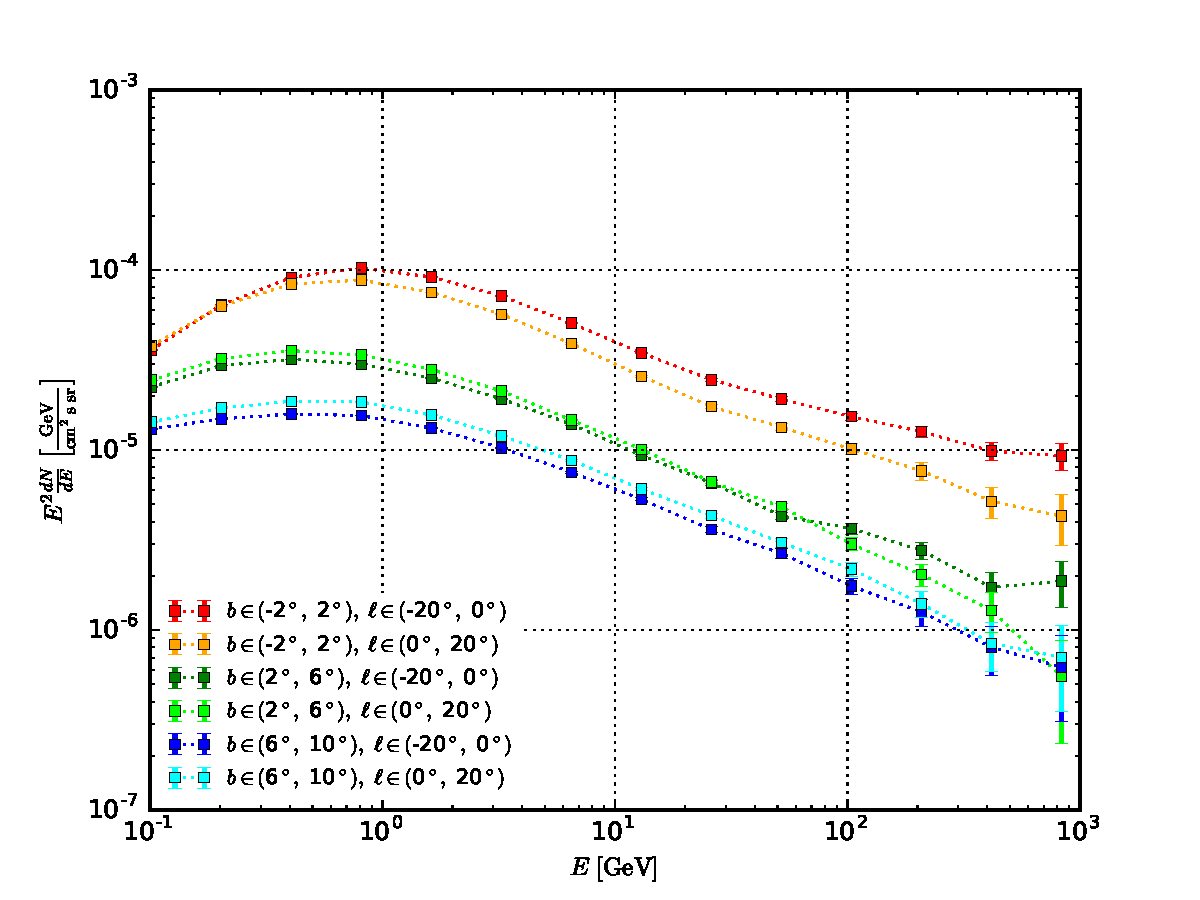
\includegraphics[width=.95\textwidth]{SED_1_top.pdf}
		\end{subfigure}%
		\hspace{-1.1cm}
		\begin{subfigure}[b]{.6\textwidth}
			\centering
			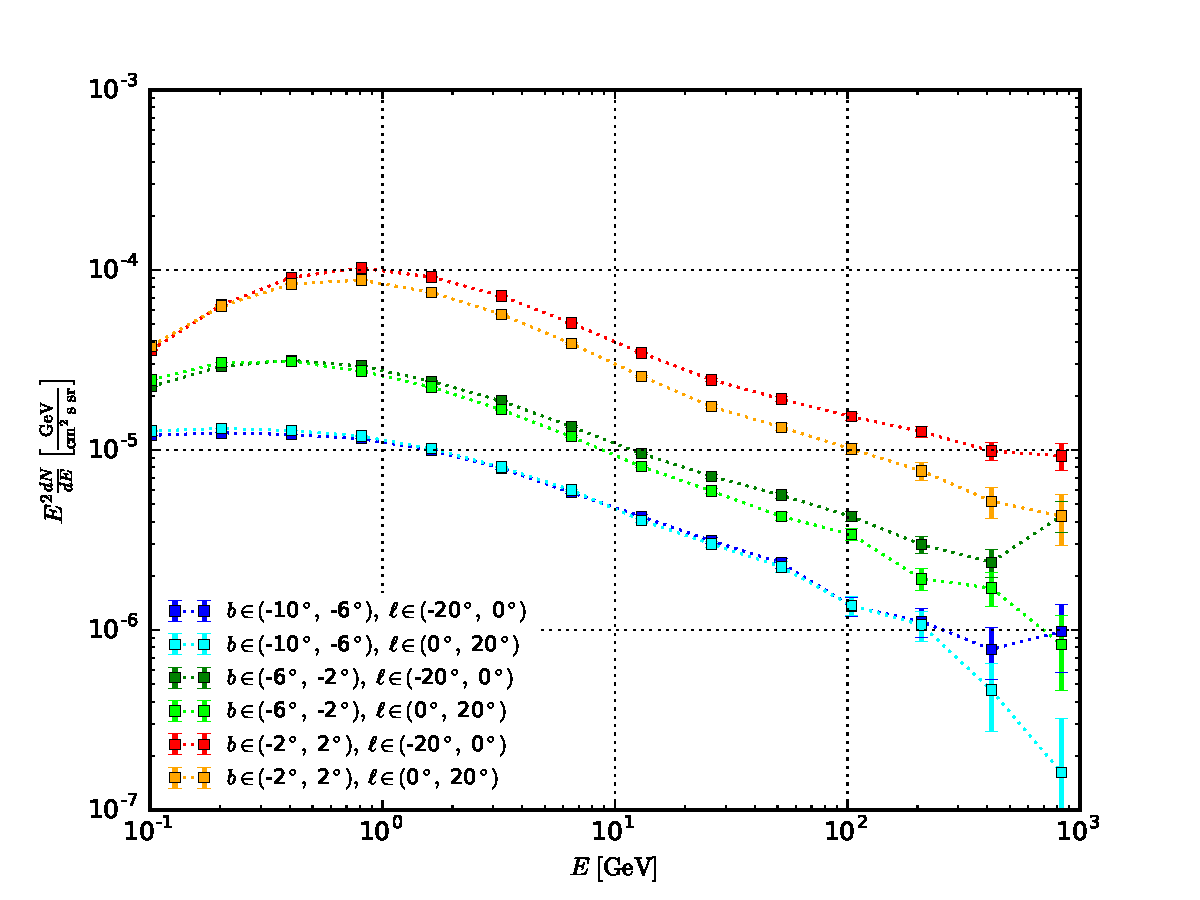
\includegraphics[width=.95\textwidth]{SED_1_bottom.pdf}
		\end{subfigure}%
}
\caption{Spectral energy distribution at low latitudes. The left plot shows the SED of the north bubble, the right plot the south bubble. The graphs for $b \in (-2^\circ,2^\circ)$ can be seen in both plots. Lighter colours indicate regions to the left, darker colours regions to the right of the Galactic center. Point sources are masked.}
\label{SED_at_low_lat}
\end{figure}\\
\\
One observes that the SED to the right of the Galactic center, i.e., $\ell \in (-20^\circ, 0^\circ)$, is clearly harder than to the left of the Galactic center, i.e., $\ell \in (0^\circ, 20^\circ)$, at almost every latitude. This confirms that there is an excess of hard emission to right of the Galactic center.





\subsubsection{Fit a single power law or add another power-law with a cutoff}

\subsection{Fit in stripes using low energy data as the background model} 
Unfortunately, the $\chi^2$-fitting procedure encounters a problem if the number of counts in one bin is zero. Therefore, a \textbf{likelihood} fit is applied to improve the performance. Since the approach to use low-energy \textit{Fermi} data seems promising, this method is kept to model the soft emission in our Galaxy. Additionally, the model is improved by another parameter $c$ that takes the isotropic gamma-ray background into account. The total model $N_{\text{model}} = k \cdot N_{\text{low}} + c$ is again fitted in $1^\circ$-latitude stripes to the data $N_{\text{high}}$. Since for the method of maximum likelihood a Poisson-distributed variable is required, instead of the integrated intensity one uses the number of photon counts in each latitude-longitude bin and each energy interval. In order to reduce the formation of holes by point sources in the residual, the lower energy interval is set to 600 MeV - 1.6 GeV. This time the region of the bubbes, i.e., $\ell \in (-20^\circ,20^\circ)$, is excluded from the fit to avoid an over-compensation of the hard emission by the model. Point sources are masked. For details on the likelihood fit see the appendix \ref{likelihood}.\\
\begin{figure}[h!]
    \begin{subfigure}{0.5\textwidth}
    	\centering
        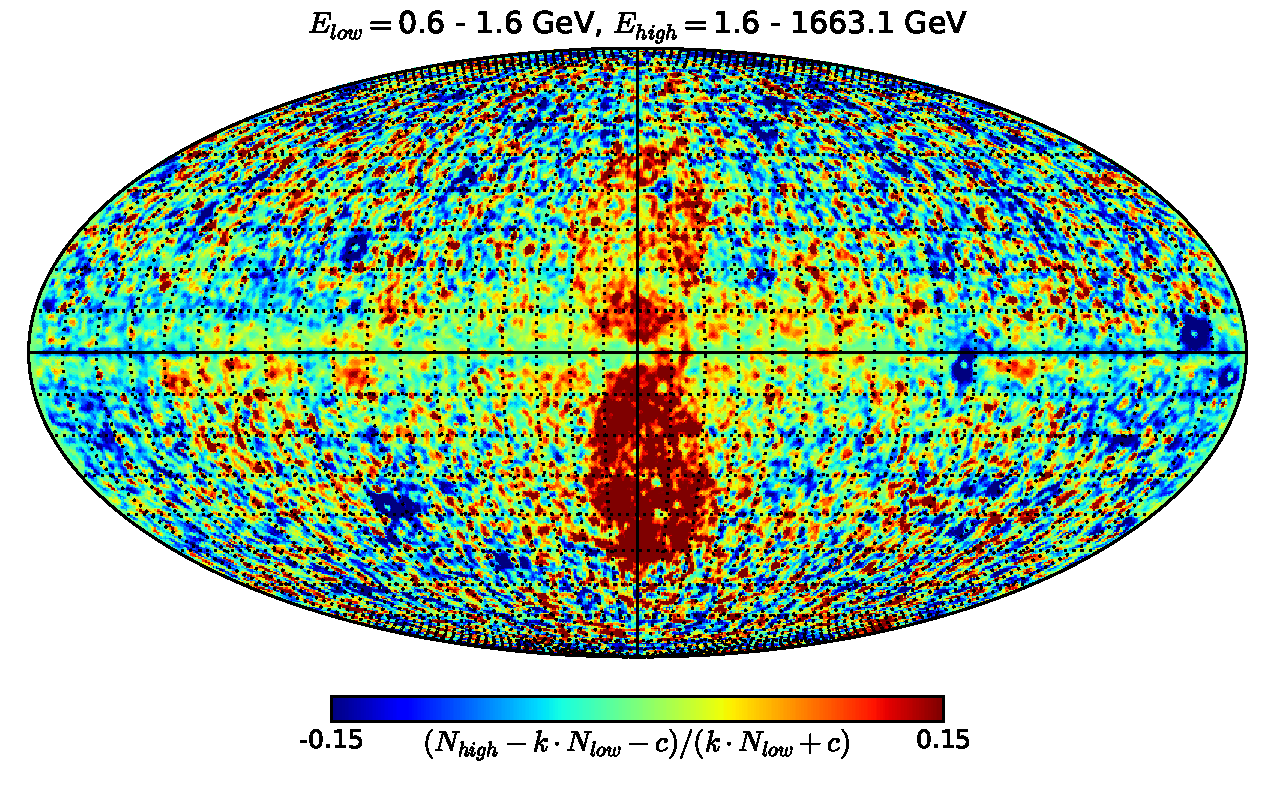
\includegraphics[width=\textwidth]{FitE_mollweide_at_0-1_to_1-1663015.pdf}
    \end{subfigure}
    \begin{subfigure}{0.5\textwidth}
    	\centering
        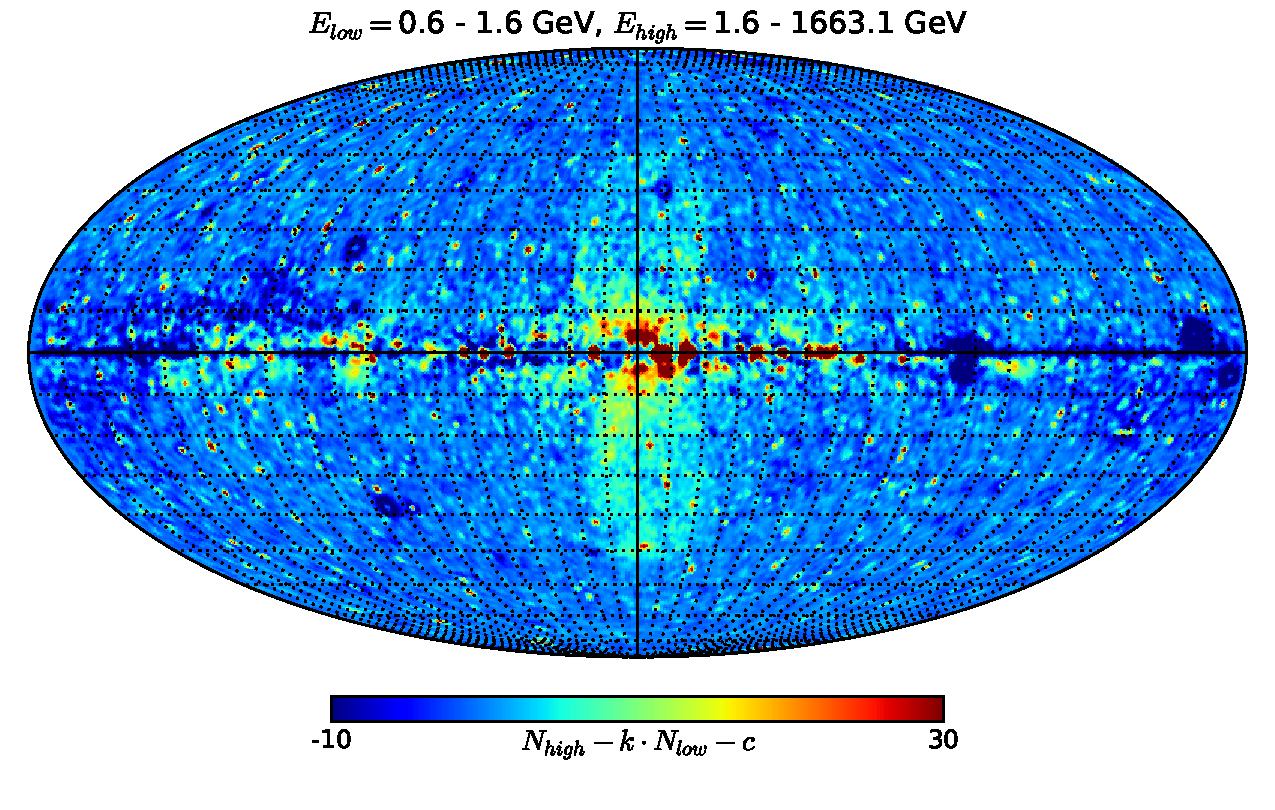
\includegraphics[width=\textwidth]{FitE_mollweide_at_0-1_to_1-1663_nonorm.pdf}
    \end{subfigure} 
    \caption{Residual photon-counts map after subtraction of the model, normalized (left) and not normalized by the model (right). The energy range of the model is given by $E_{\text{high}}$, the energy range of the data by $E_{\text{low}}$. The map is smoothed with a Gaussian of $5^\circ$ FWHM. Point sources are masked.}
    \label{lowE_likelihood_mollweide}
\end{figure}\\
The resulting residual photon-counts map is shown in Figure \ref{lowE_likelihood_mollweide}. The \textit{Fermi} bubbles are again clearly visible. In the left map of Figure \ref{lowE_likelihood_mollweide} the residual has been normalized by the model, revealing the bubbles again as two lobes of hard spectra. The right map of Figure \ref{lowE_likelihood_mollweide} shows the total residual photon counts, making regions of high-excess emission visible. One excess to the right of the Galactic center in the Galactic plane at $\ell = -5^\circ$ attracts attention. It seems to be connected to the bubbles by a band of hard emission. Further to the right another excess emission stands out at $\ell = -15^\circ$. The Galactic center itself appears to have a comparatively soft spectrum.\\
\\
In Figure \ref{lowE_likelihood_profiles} the model is further analyzed at low latitudes. Shown are the longitudinal profiles of photon counts at $|b| < 10^\circ$ in $\Delta b = 4^\circ$ stripes. The two excesses that were discovered in the all-sky map are again visible at $b \in (-2^\circ, 2^\circ)$, and $\ell = -5^\circ$ and $\ell = -15^\circ$, respectively. The two stripes below the Galactic plane, i.e., $b \in (10^\circ, -2^\circ)$, indicated by darker colours, show both an excess at the Galactic center and one at around $\ell = -8^\circ$ to the right of the Galactic center. On the other hand, the two stripes above the Galactic plane, i.e., $b \in (2^\circ, 10^\circ)$, indicated by lighter colours, possess excessive hard emission centered around the Galactic center.\\
\\
\begin{figure}[t]
	\centering
	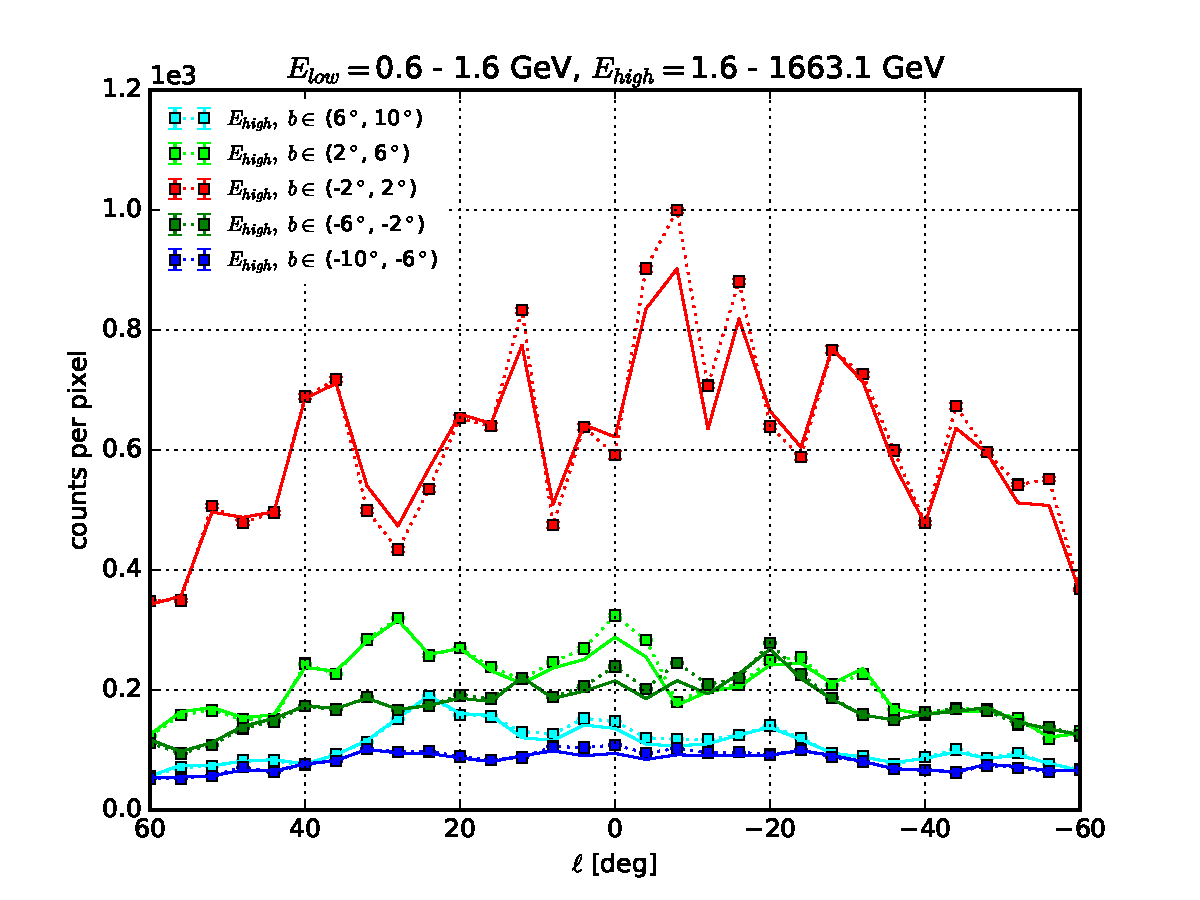
\includegraphics[width=0.7\textwidth]{FitE_profile_plot_at_0-1_to_1-1663.pdf}
    \caption{Longitudinal profiles of photon counts per pixel at small latitudes. Darker colours indicate latitude stripes above the Galactic plane, lighter colours indicate latitude stripes below. The region of the bubbles, i.e., $\ell \in (-20^\circ,20^\circ)$, is excluded from the fit. Point sources are masked.}
    \label{lowE_likelihood_profiles}
\end{figure}
Accordingly, all modelling done in this work indicates an assymmetry with respect to the Galactic center. Hard gamma radiation seems to be more abundant to the right of the Galactic center. Since the spectrum of the \textit{Fermi} bubbles themselves is very hard, it is reasonable to look out for regions of extraordinary hard spectra in the Galactic plane. They might be related to the origin of the \textit{Fermi} bubbles.





\subsection{``Model'' the bubbles as a collection of rectangles}

The model of the previous section is extended by a collection of rectangles, that cover the bubbles roughly. The low-energy data, isotropic background and rectangles are fitted in $4^\circ$-latitude stripes. The rectangle in each stripe is divided into an eastern and a western part; each part is fitted separately to the data.\\
Figure \ref{boxes_fit} (left) shows the residual in Mollweide projection for two types of ``boxes'': The bubbles are modelled first by rectangles that cover the region from $-20^\circ$ to $20^\circ$ in every latitude stripe (first row in Fig. \ref{boxes_fit}). Though, this ``model'' is very rough, it eats large parts of the positive bubble residual. \\
The second ``model'' has the following shape, tracing the bubbles a little better:

\begin{description}
\item[$-180^\circ < b < -14^\circ$:] Rectangle from $-20^\circ$ to $16^\circ$,
\item[$-14^\circ < b < 10^\circ$:] Rectangle from $-10^\circ$ to $10^\circ$,
\item[$-10^\circ < b < -2^\circ$:] Rectangle from $-4^\circ$ to $4^\circ$,
\item[$-2^\circ < b < 18^\circ$:] Rectangle from $-8^\circ$ to $8^\circ$,
\item[$18^\circ < b < 180^\circ$:] Rectangle from $-20^\circ$ to $16^\circ$.
\end{description}
The sizes have been chosen such that the fit works best.
 

\begin{figure}[H]
	\makebox[\linewidth][c]{%
	\begin{subfigure}[b]{.5\textwidth}
		\centering
		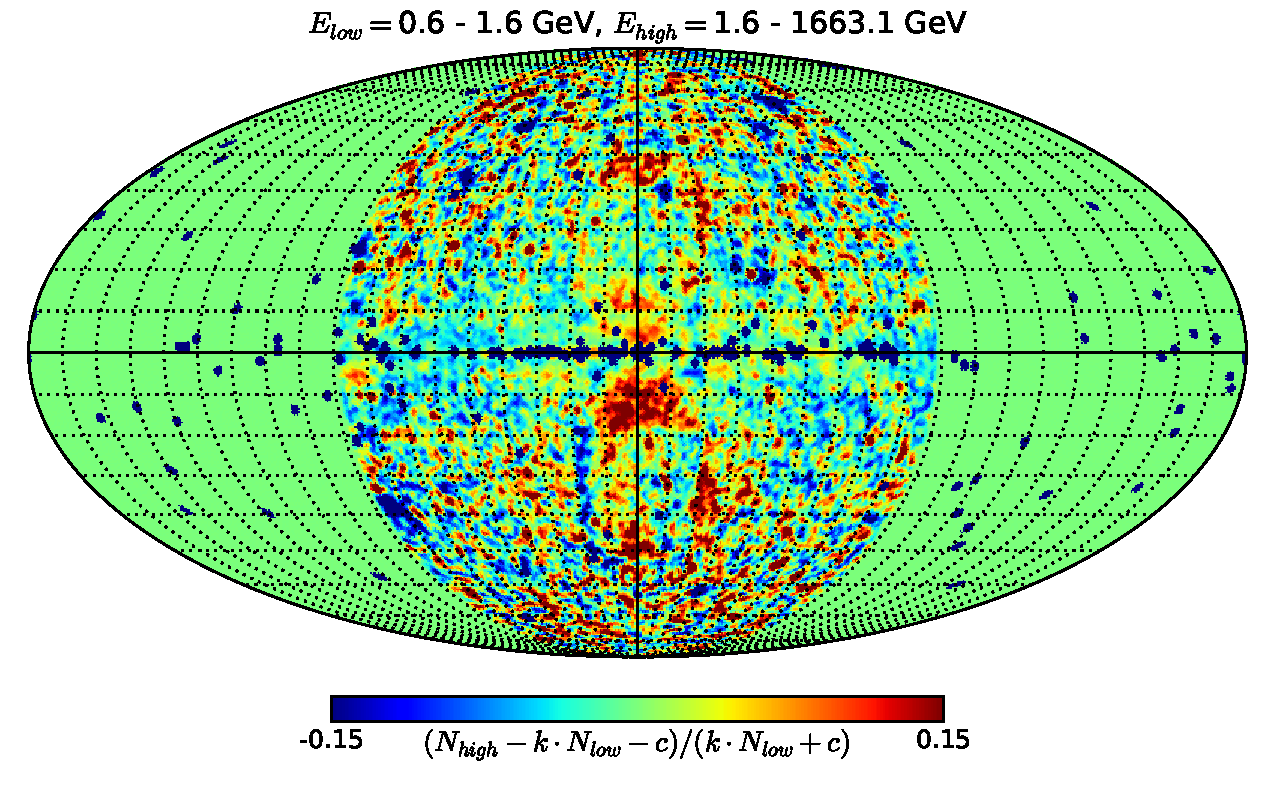
\includegraphics[width=.95\textwidth]{FitE_mollweide_at_0-1_to_1-1663_norm_new.pdf}
	\end{subfigure}%
	\begin{subfigure}[b]{.5\textwidth}
		\centering
		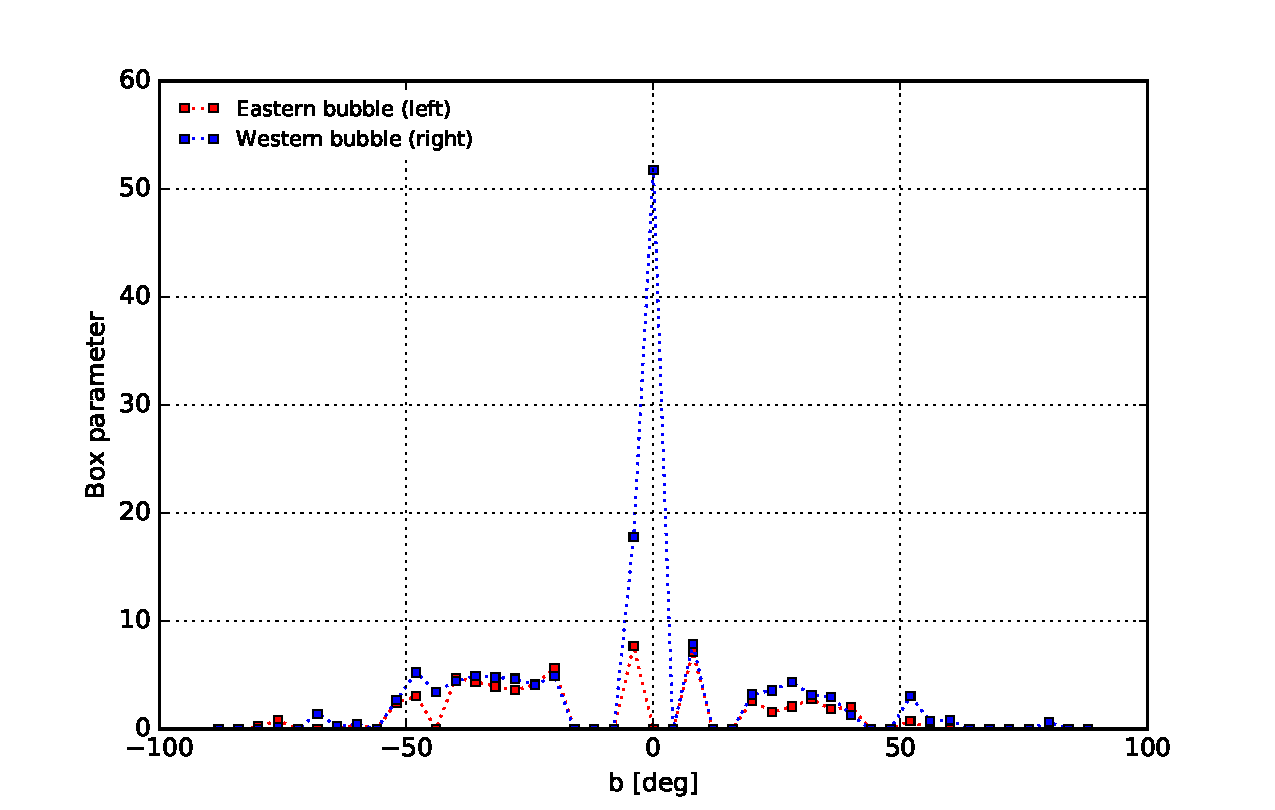
\includegraphics[width=.95\textwidth]{FitE_boxprof_at_0-1_to_1-1663_norm_new.pdf}
	\end{subfigure}
	%\vspace*{-3cm}
	}\\
	\makebox[\linewidth][c]{%
	\vspace*{-3cm}
	\begin{subfigure}[b]{.5\textwidth}
		\centering
		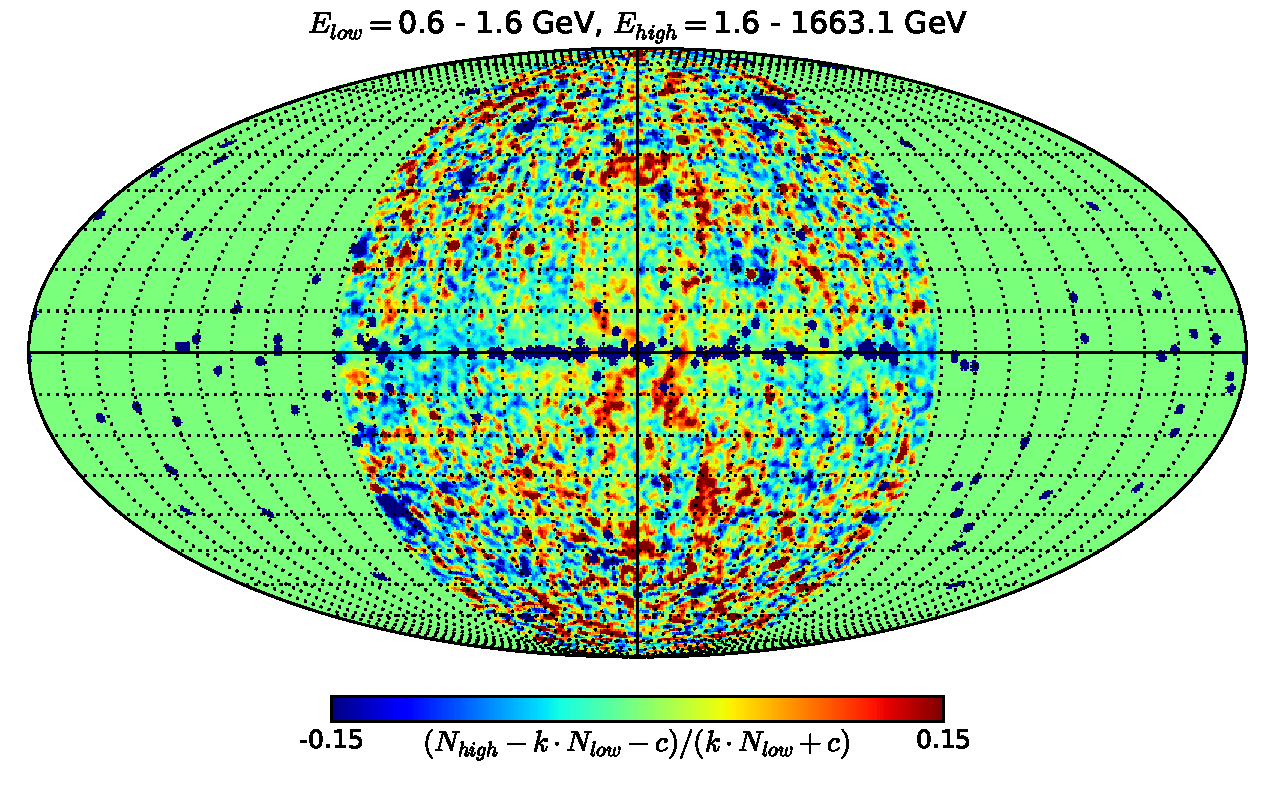
\includegraphics[width=.95\textwidth]{FitE_mollweide_at_0-1_to_1-1663_norm_fitbubshape.pdf}
	\end{subfigure}%
	\begin{subfigure}[b]{.5\textwidth}
		\centering
		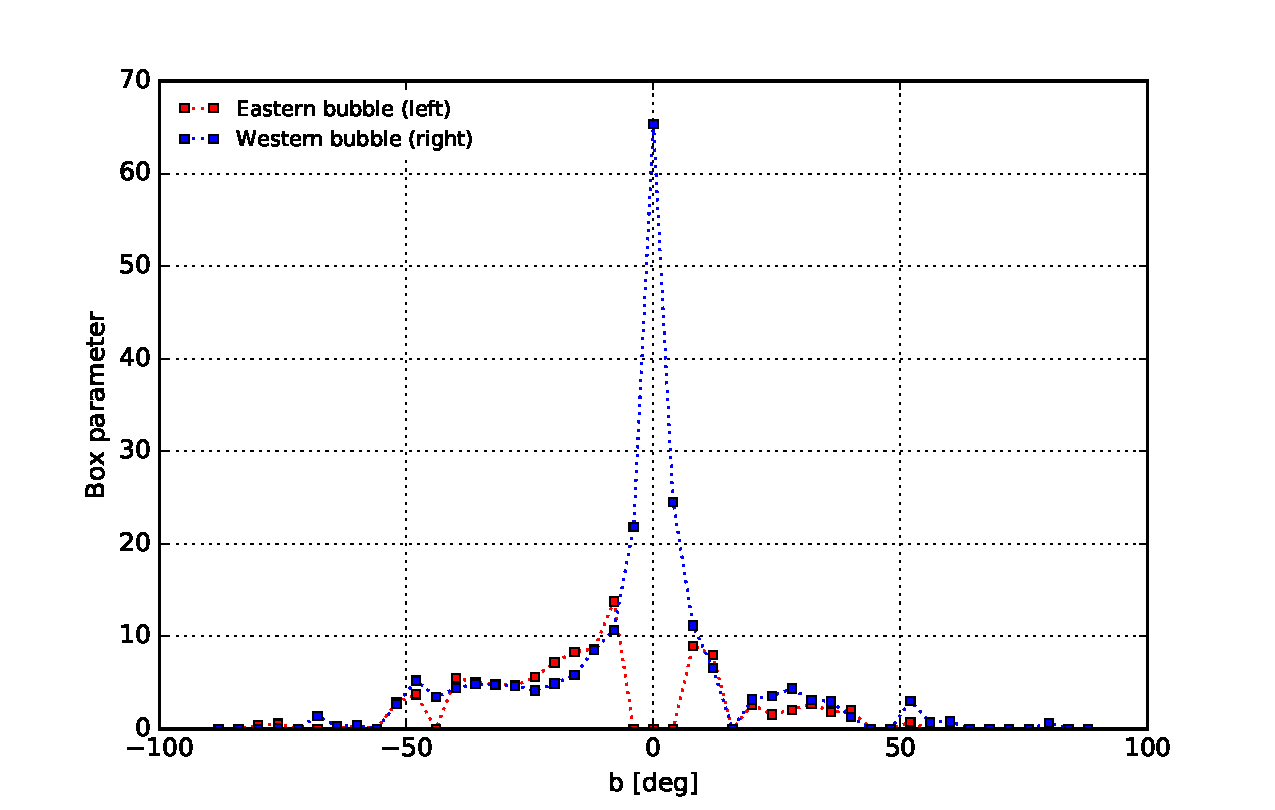
\includegraphics[width=.95\textwidth]{FitE_boxprof_at_0-1_to_1-1663_norm_fitbubshape.pdf}
	\end{subfigure}%
	}\\
\caption{Residual of low-energy data model with rectangles in Mollweide projection (left) and corresponding latitude profile of the box parameter (right), i.e. the fitting parameter of the rectangle. The rectangles west and east have been fitted independently. \textit{Top row:} Rectangles have the same length in every latitude stripe ($-20^\circ, 20^\circ$), \textit{bottom row:} Rectangles have sizes as indicated in the text, adapted to the shape of the \Fermi bubbles. Point sources have been masked. The high-energy data has been smoothed with a Gaussian of $0.5^\circ$ FWHM to compensate for the worse resolution at low energies. Only data with $|b| < 90^\circ$ is taken into account.}
\label{boxes_fit}
\end{figure}






\subsection{Use GALPROP Galactic model instead of low-energy bins}



\section{Morphology}

\subsection{Residuals at different energies}

\newpage
\begin{figure}[H]
	\makebox[\linewidth][c]{%
	\begin{subfigure}[b]{.5\textwidth}
		\centering
		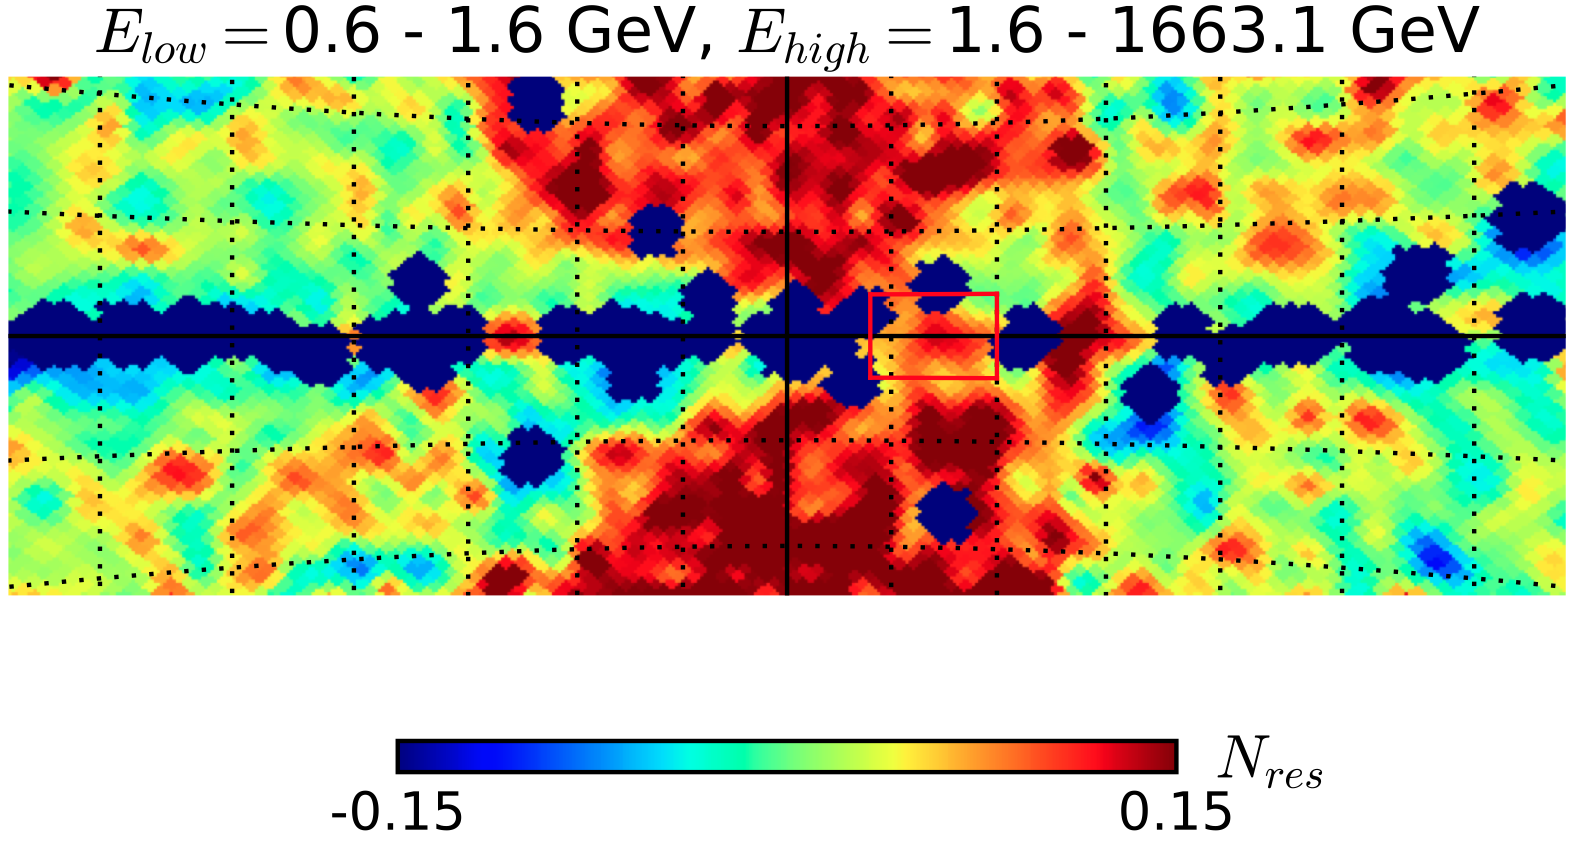
\includegraphics[width=.95\textwidth]{gnomview}
		\vspace*{1cm}
	\end{subfigure}%
	\begin{subfigure}[b]{.5\textwidth}
		\centering
		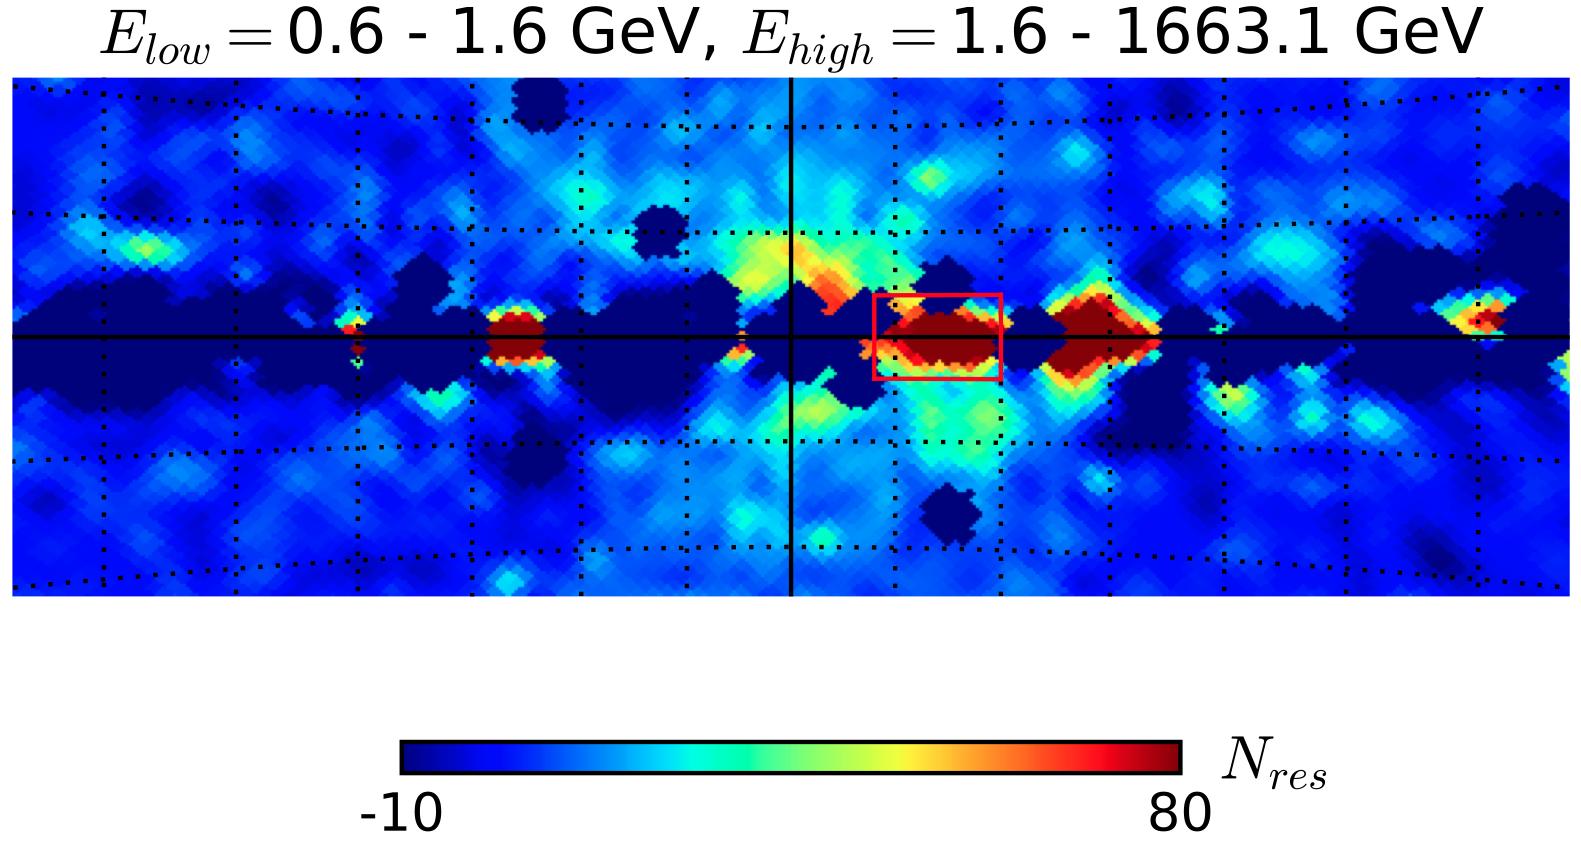
\includegraphics[width=.95\textwidth]{gnomview_nonorm}
		\vspace*{1cm}
	\end{subfigure}%
	}\\
	\vspace*{1cm}
	\makebox[\linewidth][c]{%
	\begin{subfigure}[b]{.5\textwidth}
		\centering
		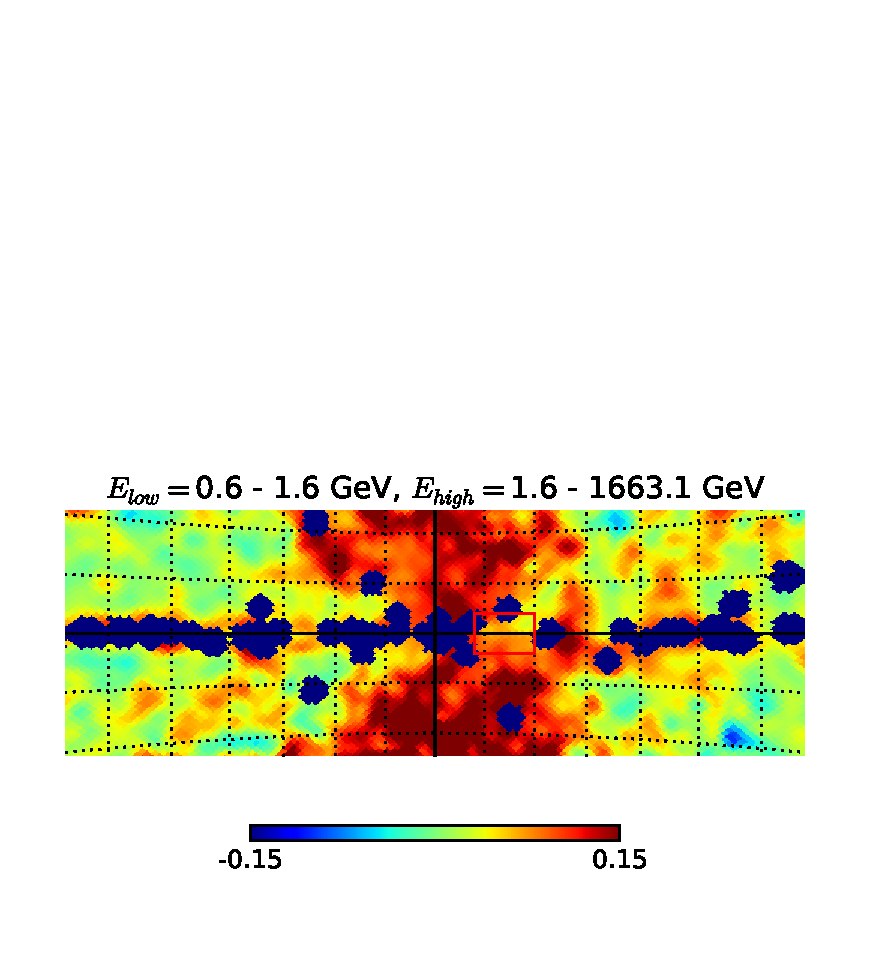
\includegraphics[width=.95\textwidth]{gnomview_highEsmooth}
	\end{subfigure}%
	\begin{subfigure}[b]{.5\textwidth}
		\centering
		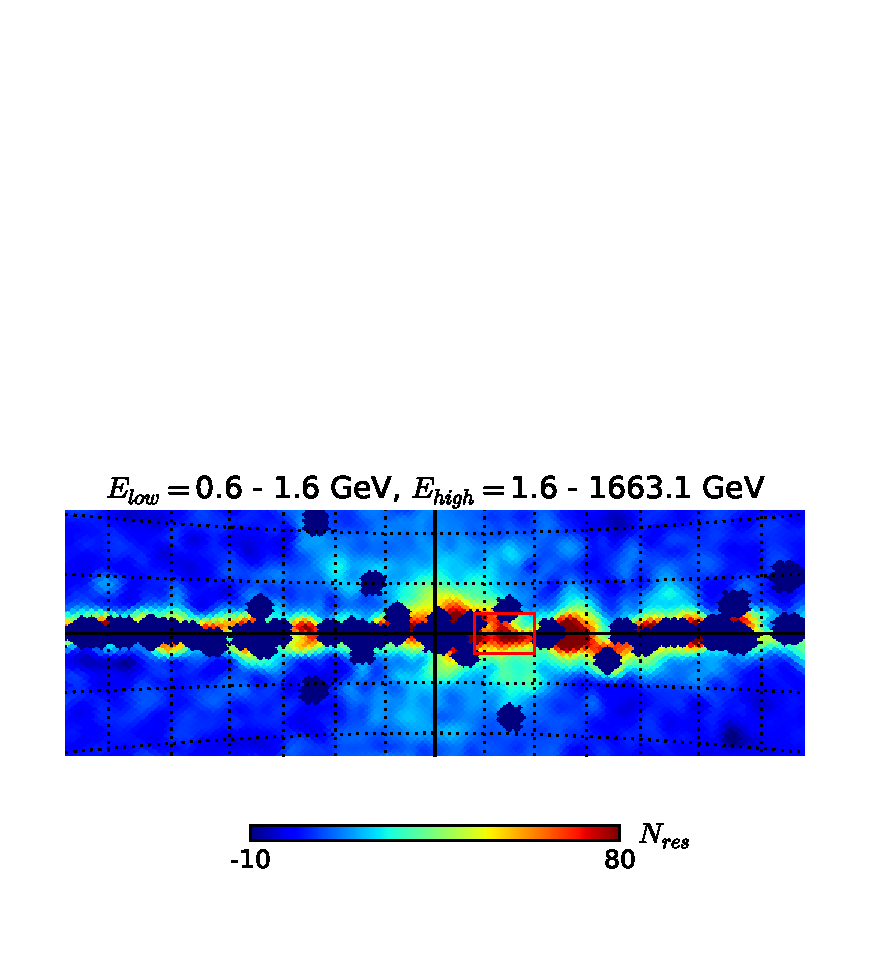
\includegraphics[width=.95\textwidth]{gnomview_highEsmooth_nonorm}
	\end{subfigure}%
	}\\
		\makebox[\linewidth][c]{%
	\begin{subfigure}[b]{.5\textwidth}
		\centering
		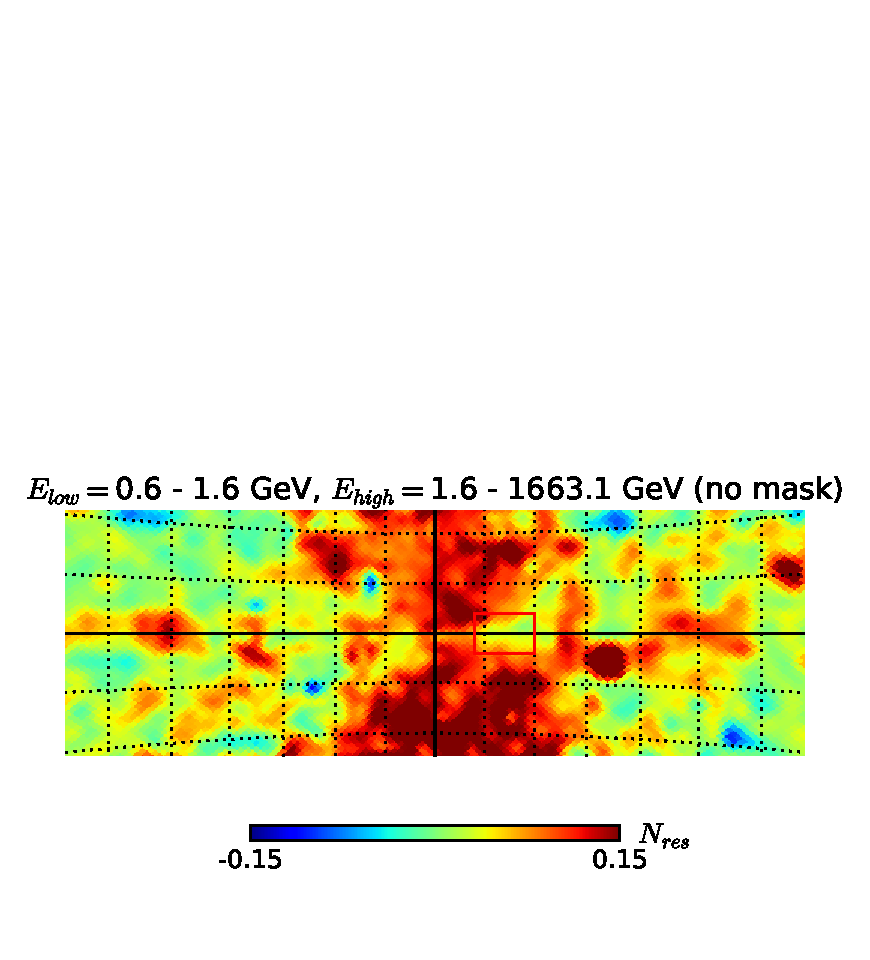
\includegraphics[width=.95\textwidth]{gnomview_highEsmooth_nomask}
	\end{subfigure}%
	\begin{subfigure}[b]{.5\textwidth}
		\centering
		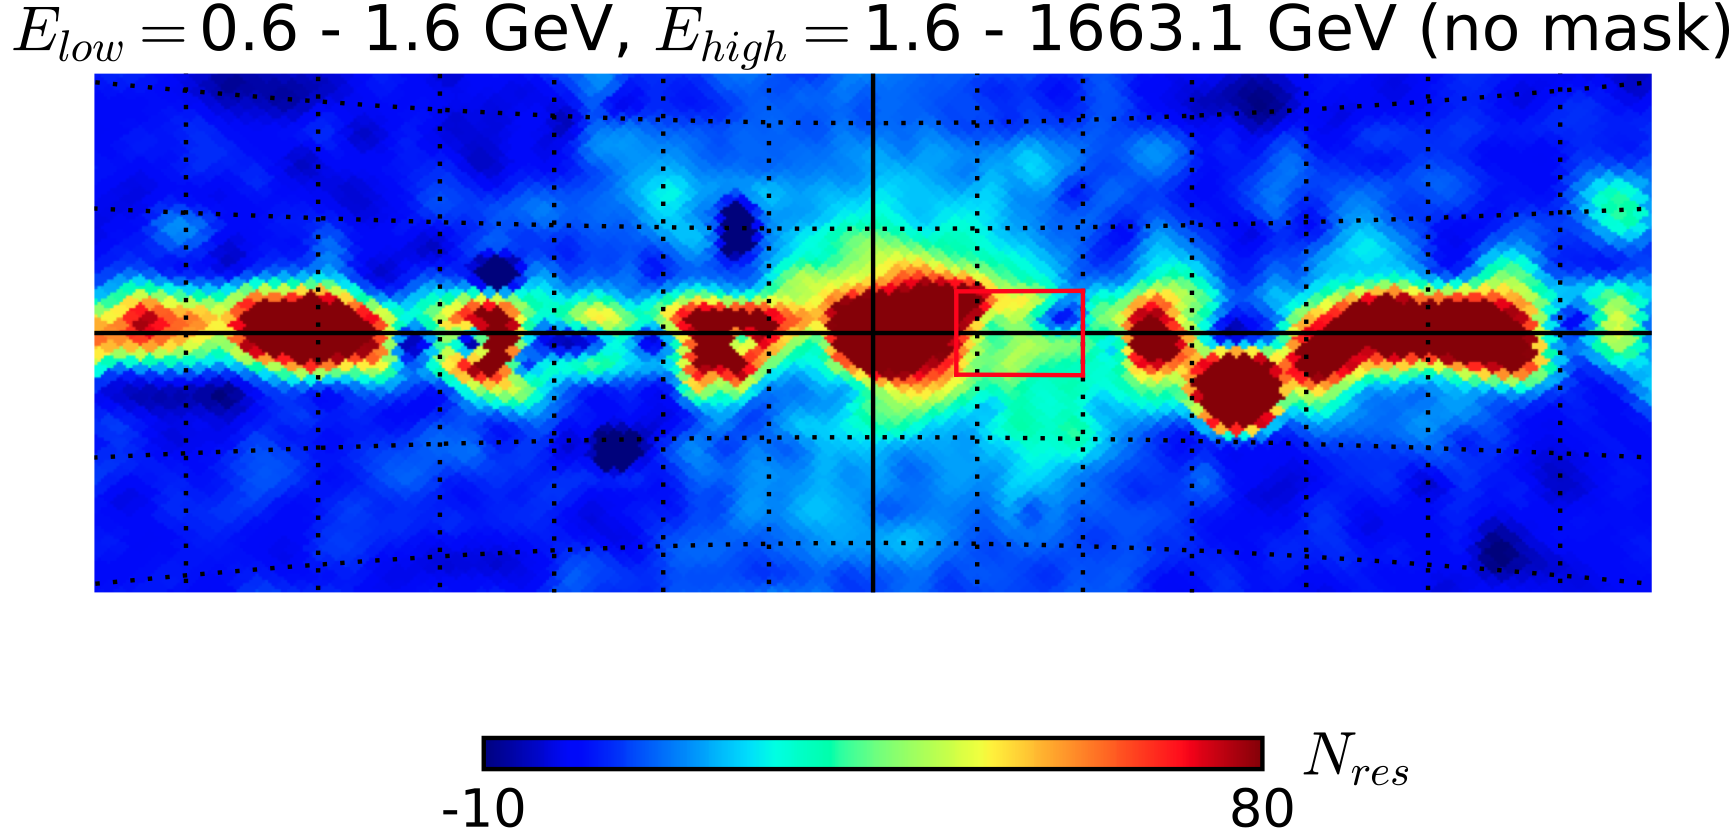
\includegraphics[width=.95\textwidth]{gnomview_highEsmooth_nonorm_nomask}
	\end{subfigure}%
	}\\
\caption{Residual photon-counts maps of the Galactic plane normalized (left) and not normalized (right). \textit{First row:} Point sources are masked and shown as the minimum value of the scale (dark blue). \textit{Second row:} The high-energy data is smoothed with a $0.5^\circ$ sigma Gaussian. \textit{Third row:} Point sources are not masked, high-energy data is smoothed. In order to avoid artefacts in the maps without mask resulting from the high fluxes of two very bright point sources on the western hemisphere (one is Crab nebula), the likelihood fit does not take into account the longitudes 0-$90^\circ$. The distance between two graticules is $5^\circ$}
\label{Fit_IC_pi0_to_ROI}
\end{figure}



\begin{figure}[h!]
	\makebox[\linewidth][c]{%
	\begin{subfigure}[b]{.5\textwidth}
		\centering
		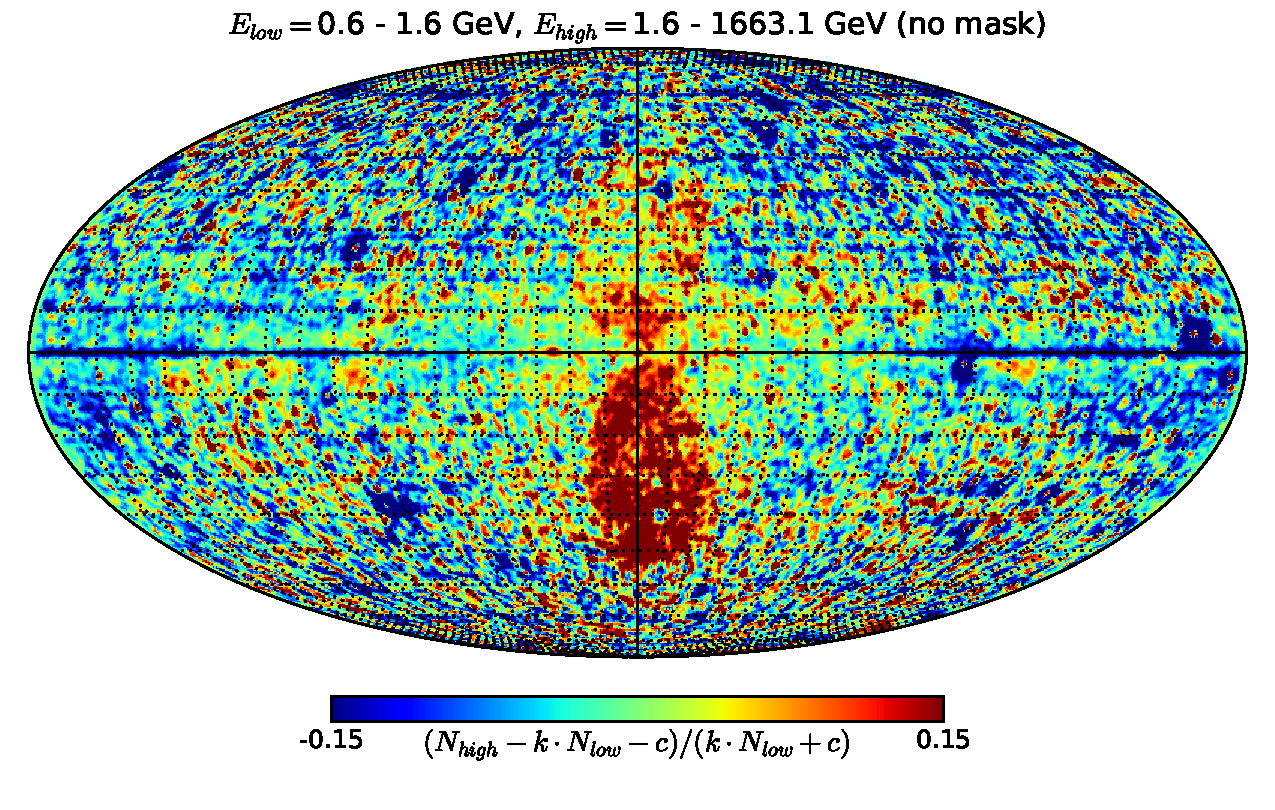
\includegraphics[width=.95\textwidth]{FitE_mollweide_at_0-1_to_1-1663_normalized_nomask.pdf}
	\end{subfigure}%
	\begin{subfigure}[b]{.5\textwidth}
		\centering
		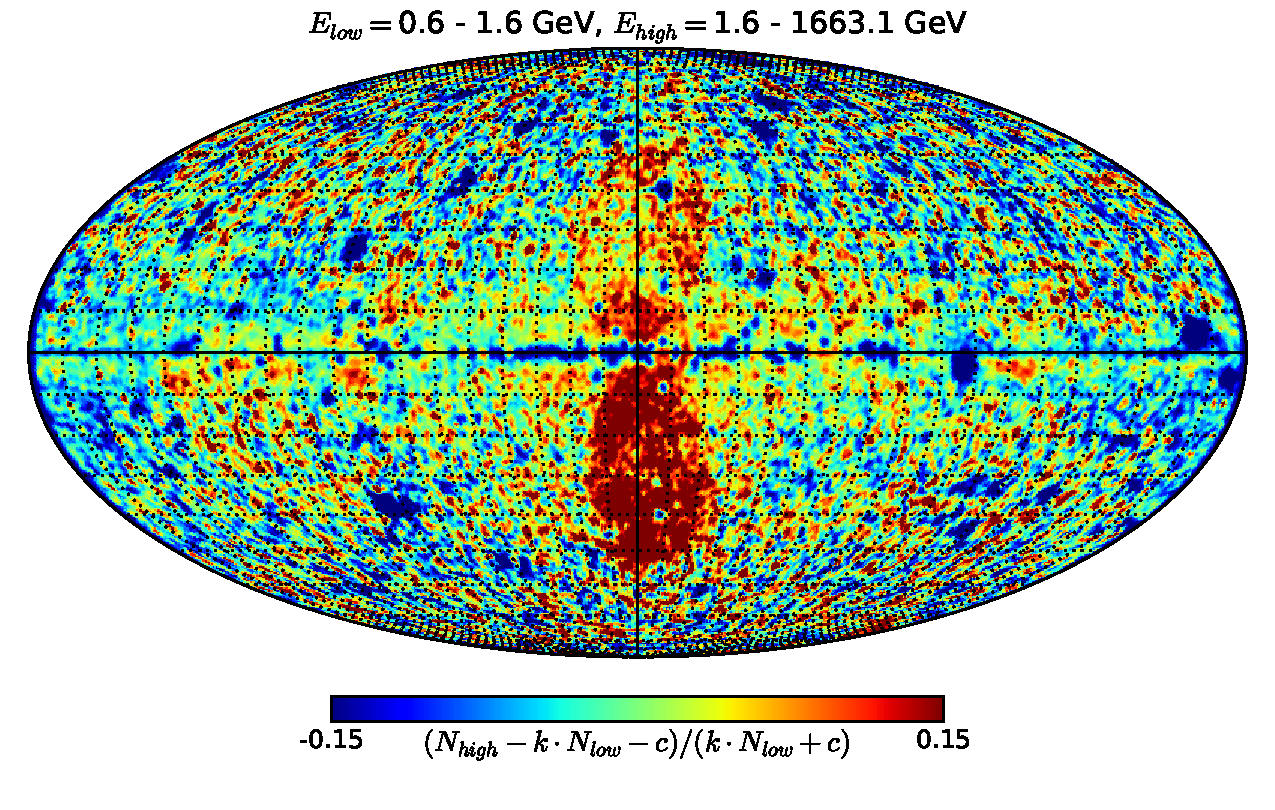
\includegraphics[width=.95\textwidth]{FitE_mollweide_at_0-1_to_1-1663_normalized_maskfilled.pdf}
	\end{subfigure}%
	}\\
	\makebox[\linewidth][c]{%
	\begin{subfigure}[b]{.5\textwidth}
		\centering
		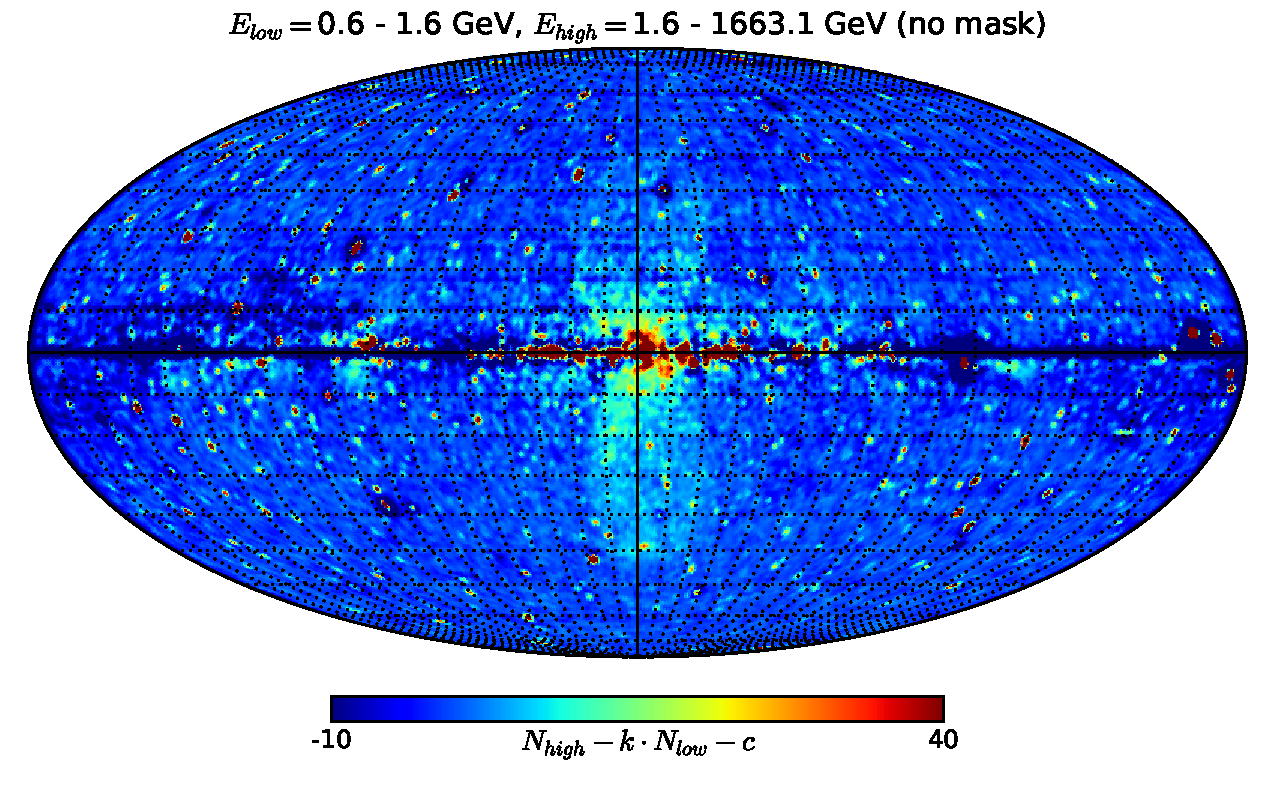
\includegraphics[width=.95\textwidth]{FitE_mollweide_at_0-1_to_1-1663_nonorm_nomask.pdf}
	\end{subfigure}%
	\begin{subfigure}[b]{.5\textwidth}
		\centering
		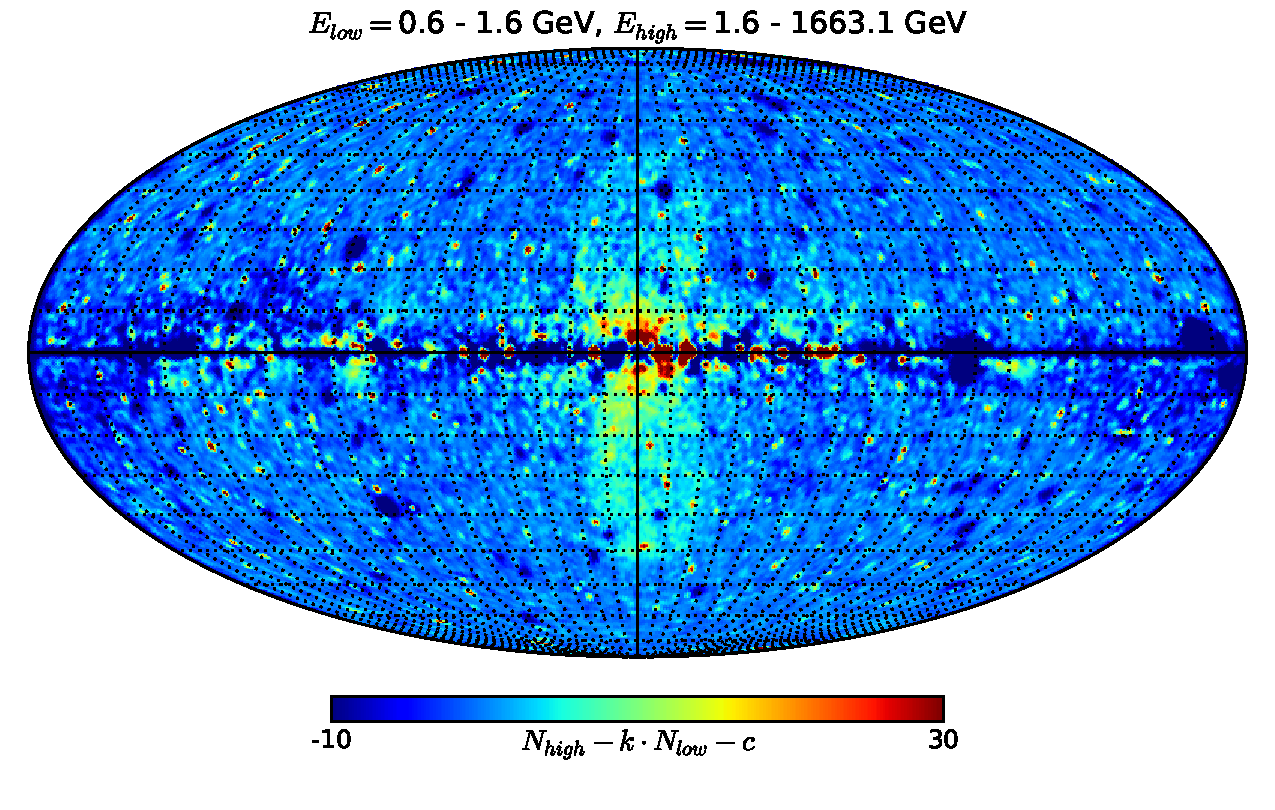
\includegraphics[width=.95\textwidth]{FitE_mollweide_at_0-1_to_1-1663_nonorm_fillmask.pdf}
	\end{subfigure}%
	}\\
\caption{Mollweide maps normalized (top) and not normalized (bottom) with (right) and without (left) point sources mask. In order to avoid artefacts in the maps without mask resulting from the high fluxes of two very bright point sources on the western hemisphere (one is Crab nebula), the likelihood fit does not take into account the longitudes 0-$90^\circ$.}
\label{Fit_IC_pi0_to_ROI}
\end{figure}




\begin{figure}[H]
	\makebox[\linewidth][c]{%
	\begin{subfigure}[b]{.5\textwidth}
		\centering
		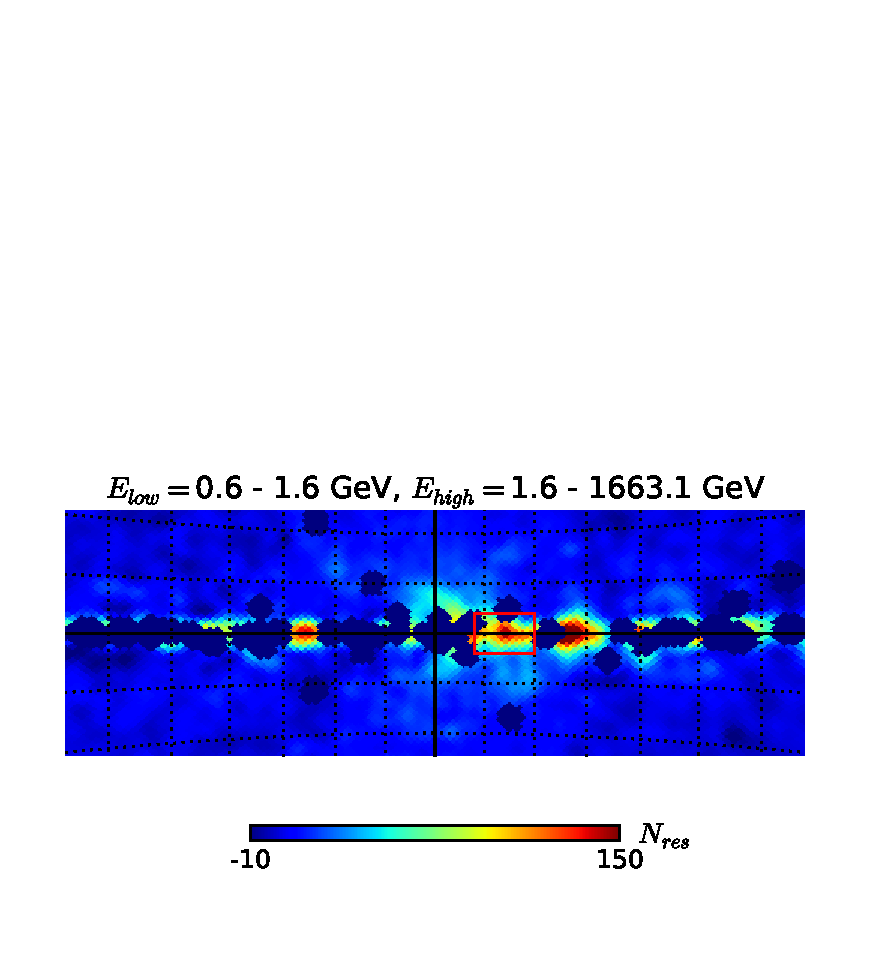
\includegraphics[width=.95\textwidth]{FitE_gnomview_at_0-1_to_1-1663_4deg}
		\vspace*{1cm}
	\end{subfigure}%
	\begin{subfigure}[b]{.5\textwidth}
		\centering
		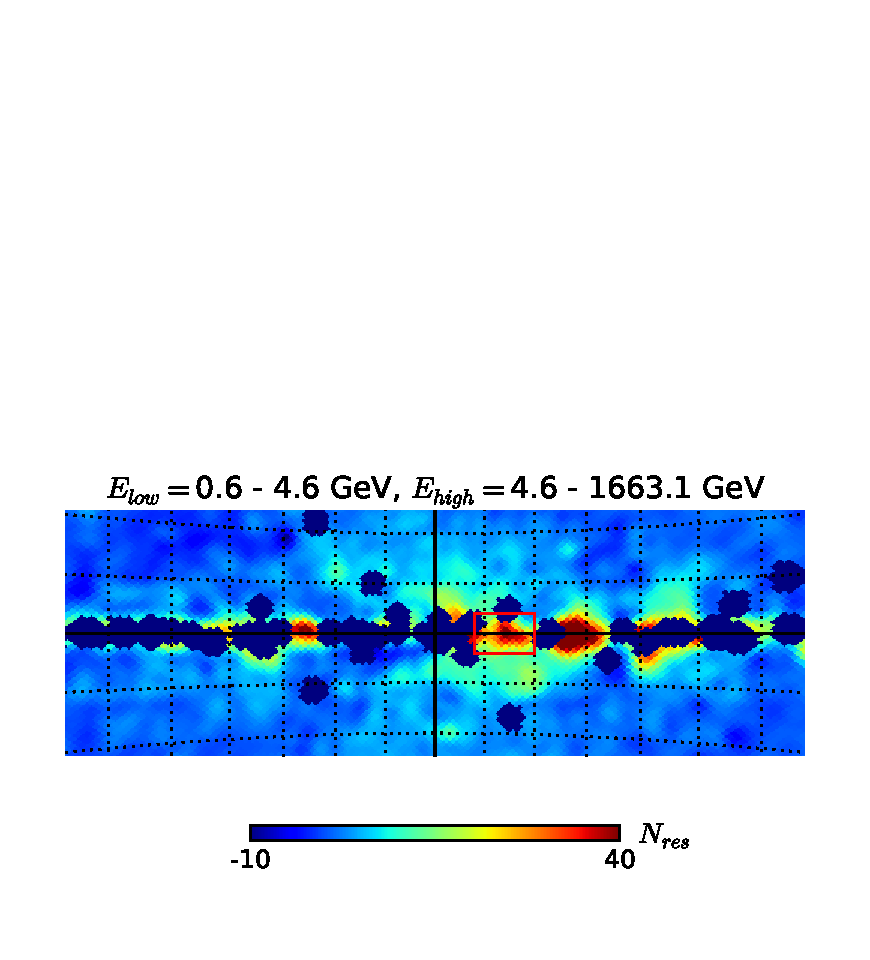
\includegraphics[width=.95\textwidth]{FitE_gnomview_at_0-4_to_4-1663_4deg}
		\vspace*{1cm}
	\end{subfigure}%
	}\\
	\makebox[\linewidth][c]{%
	\begin{subfigure}[b]{.5\textwidth}
		\centering
		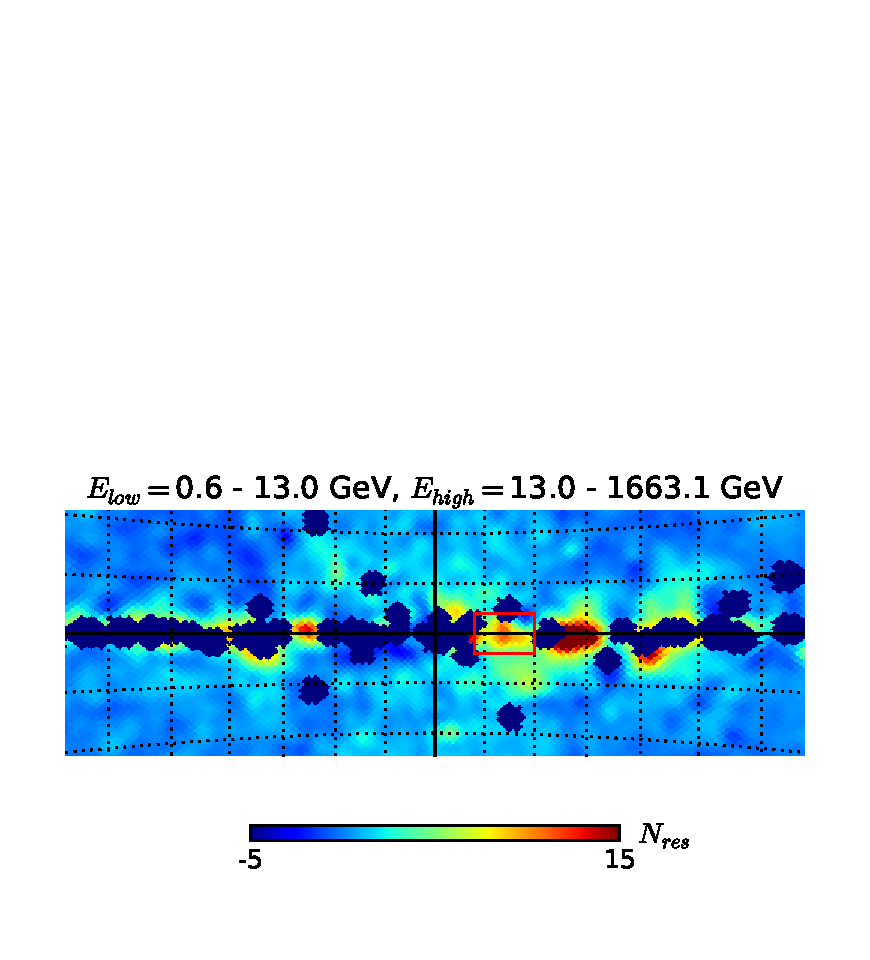
\includegraphics[width=.95\textwidth]{FitE_gnomview_at_0-12_to_12-1663_4deg}
	\end{subfigure}%
	\begin{subfigure}[b]{.5\textwidth}
		\centering
		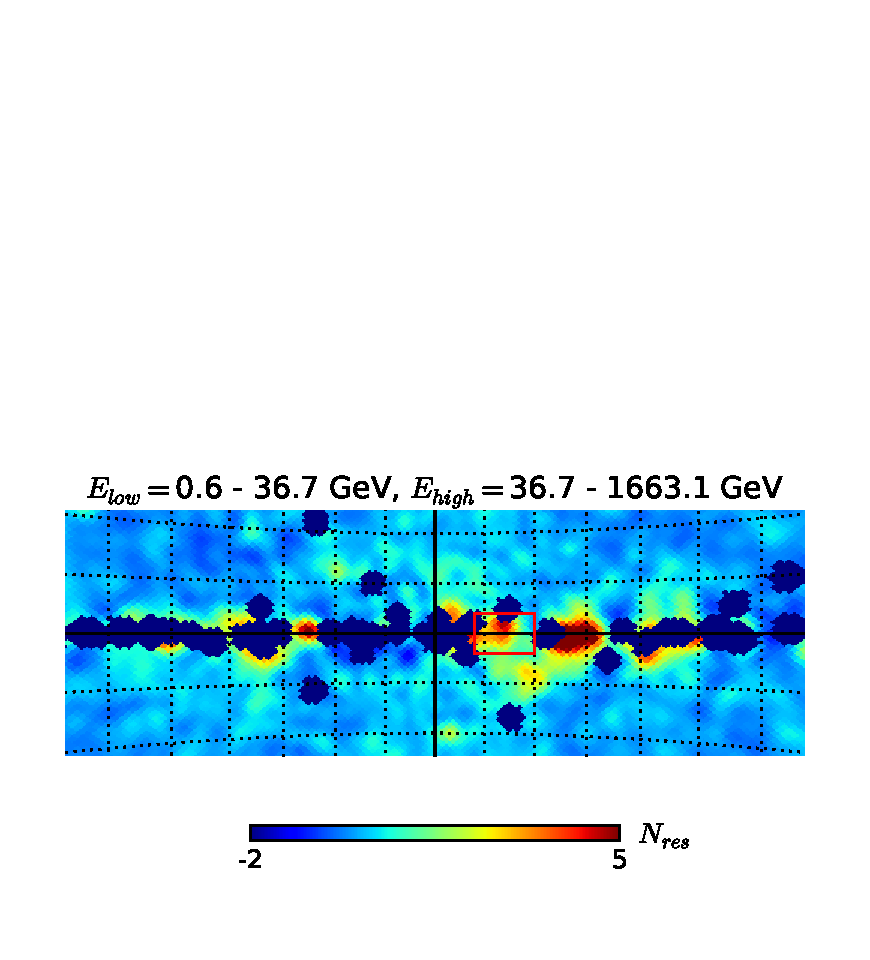
\includegraphics[width=.95\textwidth]{FitE_gnomview_at_0-36_to_36-1663_4deg}
	\end{subfigure}%
	}\\
\caption{Gnomview maps}
\label{Fit_IC_pi0_to_ROI}
\end{figure}






\newpage
\subsection{Smaller mask radius for point sources and order = 8 pixels}

\subsection{PS refitting to get unmasked residual?}


\section{Interpretation}

\subsection{$\pi^0$ and IC spectra of the residuals}


\subsubsection{The spectrum of the excess-flux region}
Besides the luminosity, also the spectral energy distribution sheds light on the emission mechanism in a gamma-ray source. Figure \ref{res_SED} (top) shows the SED of both the data and the model. To construct the model, low-energy \textit{Fermi} data and isotropic background are used. Figure \ref{res_SED} (bottom) shows the resulting residual SED. The errorbars indicate the standard deviation. One observes that only at the highest energy the SED of the data lies below the SED of the model. In the logarithmic plot, the corresponding point of the residual is negative and, therefore, only its errorbar can be seen.\\
\\
To determine the spectral index $n$, a power law 
\begin{equation}
\frac{dN}{dE} = N_0 \left( \frac{E}{E_0}\right)^{-n}
\end{equation}
is fitted to the residual data with the method of least squares. $N_0$ denotes the number of photon counts at energy $E_0$ which can be freely chosen.\\
The first and last points have not been taken into account for the fit, as the first point at 1.9 GeV is still strongly influenced by the model that contains \textit{Fermi} data below 1.6 GeV, and the last point is negative.\\
\\
The fit yields a spectral index of {\boldmath$n = 2 + \gamma = 2.16$}, where $\gamma$ denotes the spectral index of $E^2 \frac{dN}{dE}$. Typical spectral indices are, for example, {\boldmath$n = 2.4$} for IC and {\boldmath$n = 2.6 - 2.7$} for neutral pion decay. The observed spectrum is much harder. The {\boldmath$\frac{\chi^2}{n_{dof}} = 3.5$} is not so good. (???)\\
Moreover, the $\chi^2$ fit is mainly dominated by the points below 10 GeV that have very small statistical errors. If one takes a closer look at the points between 20 GeV and 1 TeV, the spectrum seems to be almost flat, i.e., $n \approx 2.0$. Since one could argue that the points below 10 GeV are still very close to the energy range of the model, i.e., 43 MeV - 1.6 GeV, the actual spectrum of the ROI could be closer to $n \approx 2.0$ than the fit would suggest. There is no apparent explanation for such a hard spectrum.\\

\begin{figure}[H]
	\centering
	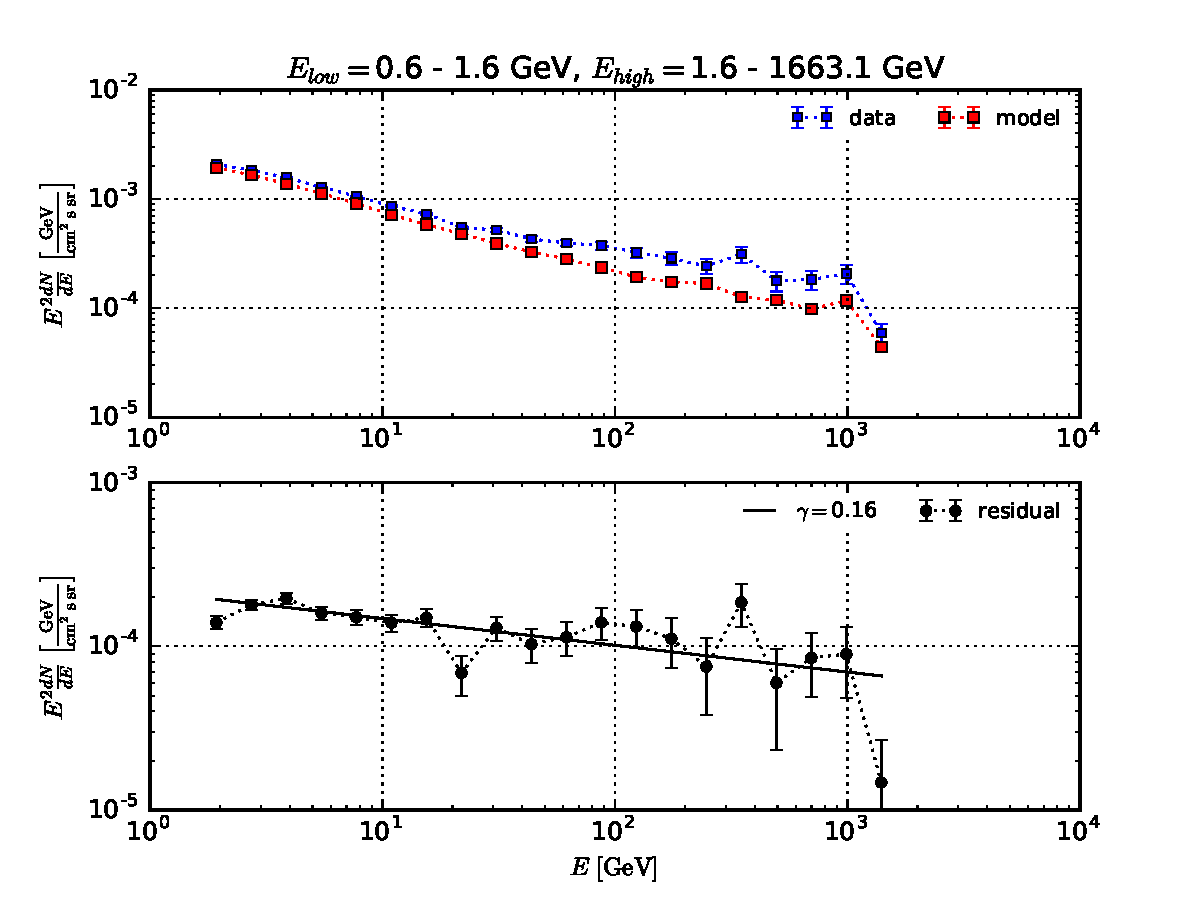
\includegraphics[width=0.8\textwidth]{Res_SED_b=(-2,2)_l=(-10,-4).pdf}
    \caption{Spectral energy distribution of the ROI. Top: SED of data (blue) and model (red). The energy range of the data is specified by $E_\text{high}$, the energy range of the model by $E_\text{low}$. Bottom: Residual SED (data - model). A power law has been fitted to the residual data, the spectral index is $n = 2 + \gamma = 2.16$. The first and last points have not been taken into account for the fit. Point sources are masked.}
    \label{res_SED}
\end{figure}
 
 
 

 
\subsubsection{The spectra of a powerlaw distribution of electrons or protons}
The two processes that have to be considered are:
\begin{enumerate}
\item Inverse Compton scattering of a distribution of relativistic electrons on the photons of the interstellar radiation field and
\item Neutral pion decay of $\pi^0$ mesons produced in collisions of relativistic protons.
\end{enumerate}
The particle spectra are modelled by simple powerlaws:
$$\left(\frac{dN}{dE}\right)_e = N_{0,IC}\ E_e^{n_{IC}},$$ 
$$\left(\frac{dN}{dp}\right)_p = N_{0,\pi^0}\ p_p^{n_{\pi^0}}.$$
The resulting photon spectra are fitted to the spectrum of the ROI with a $\chi^2$ fit. The fit result for both the total and the residual spectrum are shown in Figure \ref{Fit_IC_pi0_to_ROI}. Iminuit and scipy's fmin function yield the same results. The very similar $\chi^2$ values indicate that neither IC scattering nor $\pi^0$ decay are favoured. There is excessive radiation in the total spectrum at high energies\\
The total spectrum can be better explained by a combination of both emission mechanisms as can be seen in Figure \ref{TotalData_Sum}. The best fit result models the spectrum with a dominant $\pi^0$ emission and an additional IC contribution at higher energies. The $\chi^2$ value has decreased.
\begin{figure}[H]
	\makebox[\linewidth][c]{%
	\begin{subfigure}[b]{.65\textwidth}
		\centering
		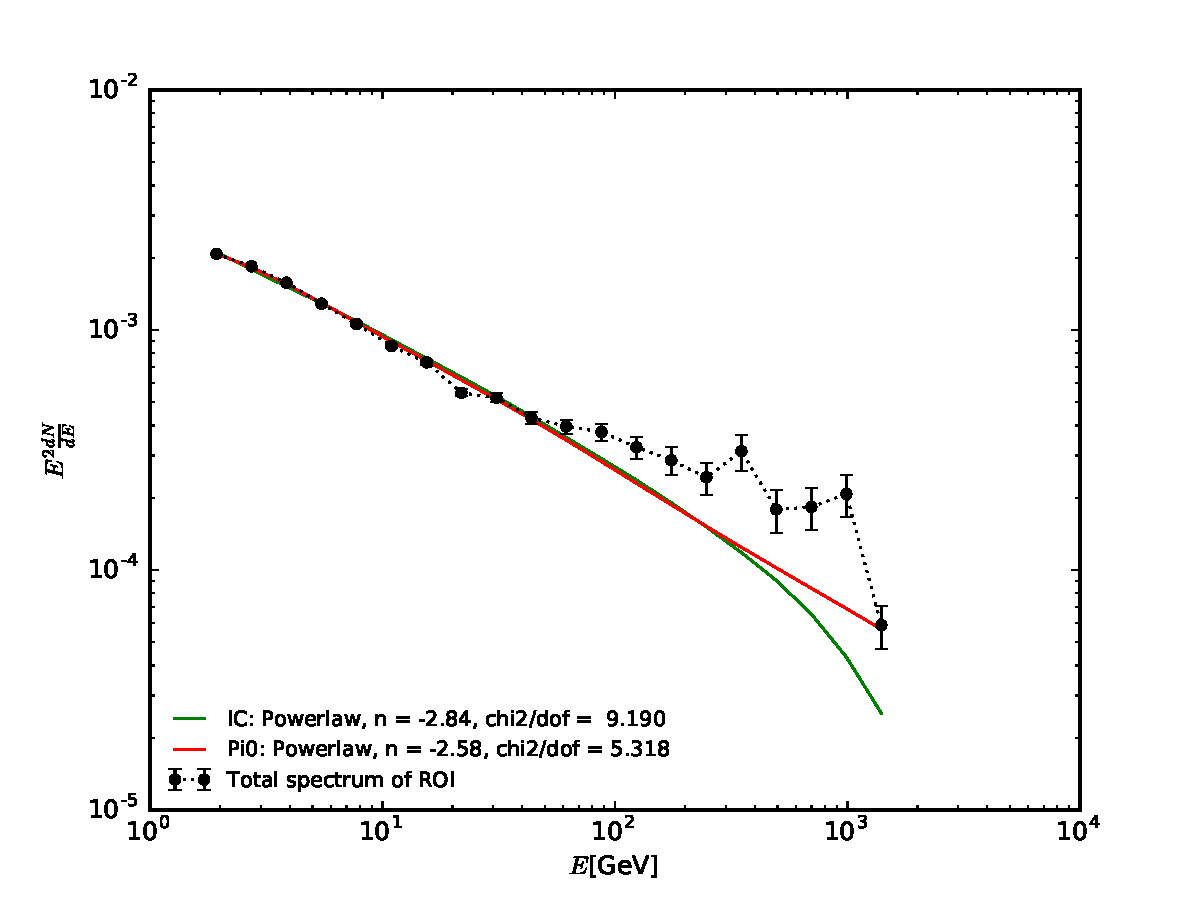
\includegraphics[width=.95\textwidth]{TotalData_IC_powerlaw_pi0-powerlaw.pdf}
	\end{subfigure}%
	\hspace*{-1.2cm}
	\begin{subfigure}[b]{.65\textwidth}
		\centering
		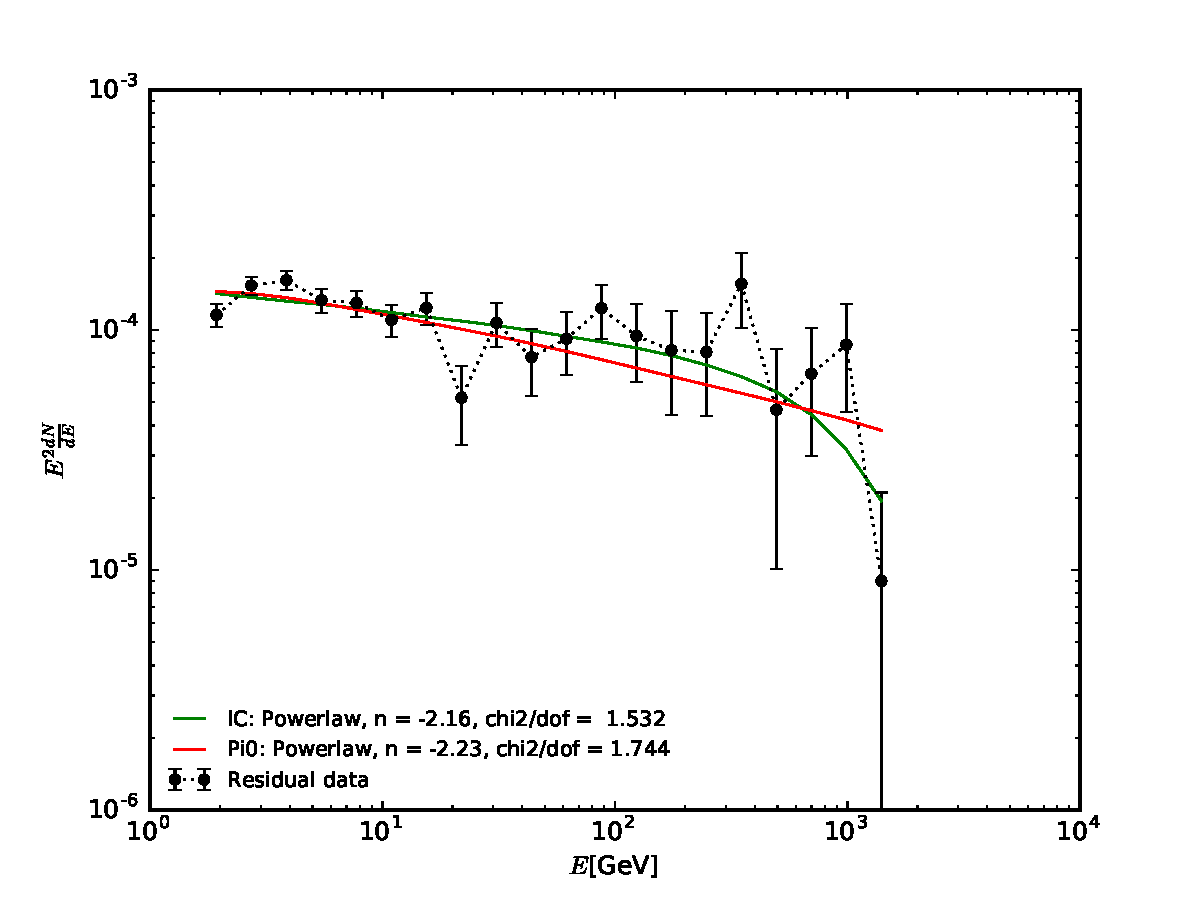
\includegraphics[width=.95\textwidth]{ResidualData_IC_powerlaw_pi0-powerlaw.pdf}
	\end{subfigure}%
	}\\
\caption{\textit{Left:} Total spectrum of the ROI. \textit{Right:} Residual spectrum using the low-energy \Fermi  data model. Both the IC and $\pi^0$ spectrum fit to the data points.}
\label{Fit_IC_pi0_to_ROI}
\end{figure}

\begin{figure}[H]
	\centering
	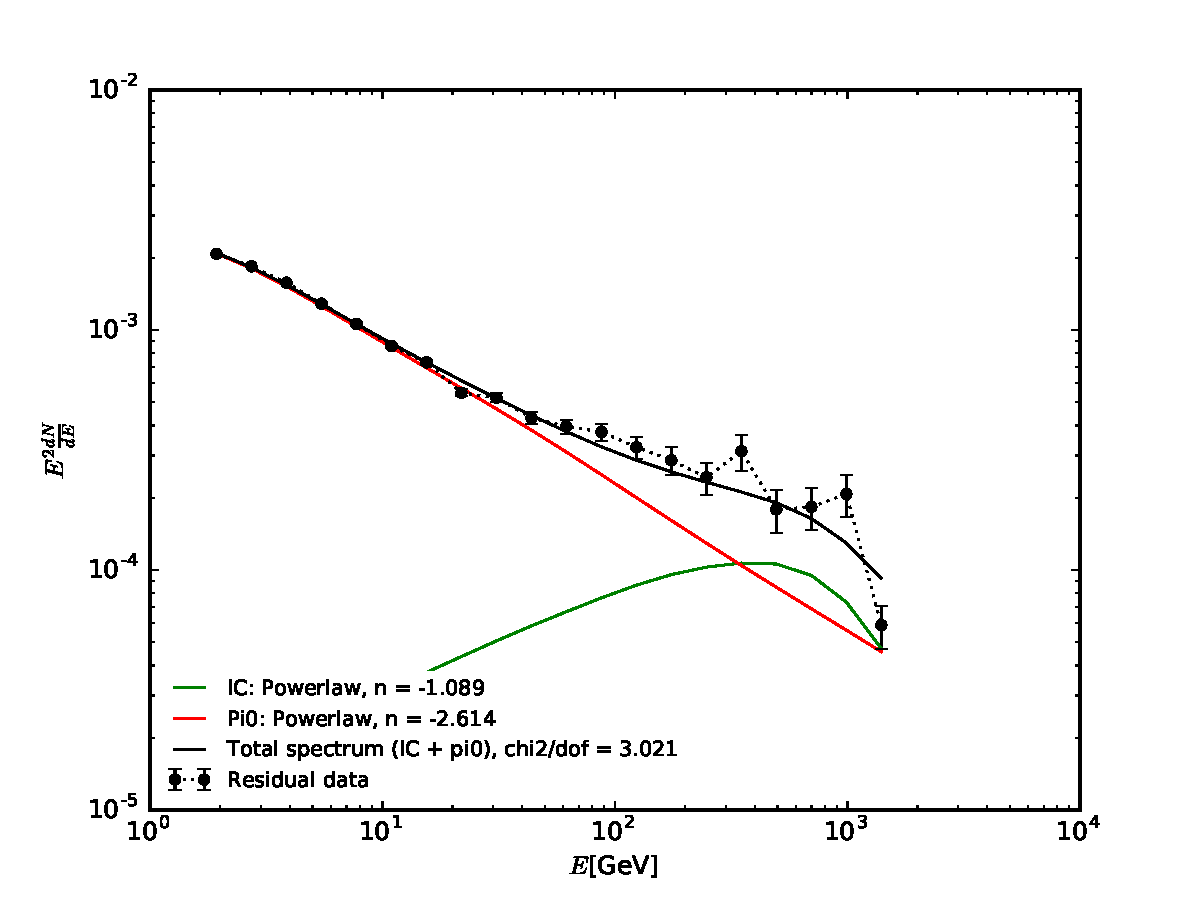
\includegraphics[width=0.8\textwidth]{TotalData_Sum_new_best.pdf}
    \caption{Sum of IC and $\pi^0$ emission fitted to the total spectrum of the ROI.}
    \label{TotalData_Sum}
\end{figure}

The best-fit parameters are:
\begin{description}
\item[Total data, independent fit:] $n_{IC} = -2.8,\ n_{\pi^0} = -2.6,\ N_{0, IC} = 9.2 \cdot 10^{14},\ N_{0, \pi^0} = 9.4 \cdot 10^{13}$
\item[Residual data, independent fit:] $n_{IC} = -2.2,\ n_{\pi^0} = -2.2,\ N_{0, IC} = 1.7 \cdot 10^{12},\ N_{0, \pi^0} = 2.2 \cdot 10^{12}$
\item[Total data, sum:] $n_{IC} = -1.1,\ n_{\pi^0} = -2.6,\ N_{0, IC} = 2.7 \cdot 10^{8},\ N_{0, \pi^0} = 1.0 \cdot 10^{14}$\\
\end{description}

\begin{figure}[H]
	\centering
	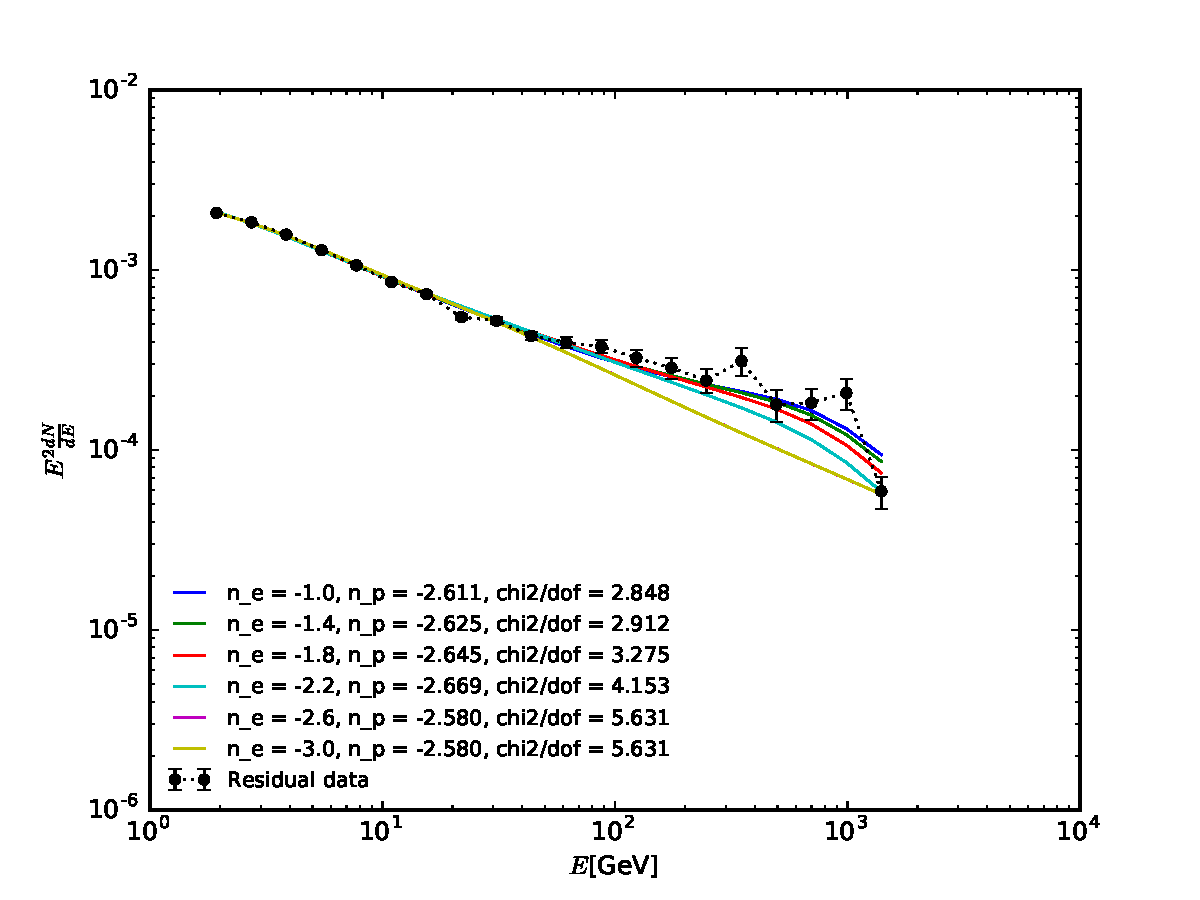
\includegraphics[width=0.8\textwidth]{TotalData_Sum_IC_n_fixed.pdf}
    \caption{Sum of IC and $\pi^0$ emission fitted to the total spectrum of the ROI for different electron spectral indices.}
    \label{TotalData_Sum}
\end{figure}





\subsubsection{Does the powerlaw have a cutoff?}
A simple powerlaw is clearly favoured over a powerlaw with cutoff. This can be seen from the decreasing $\chi^2$ value with increasing cutoff energy in Figure \ref{Cutoff_energies}. 
\begin{figure}[H]
	\makebox[\linewidth][c]{%
	\begin{subfigure}[b]{.65\textwidth}
		\centering
		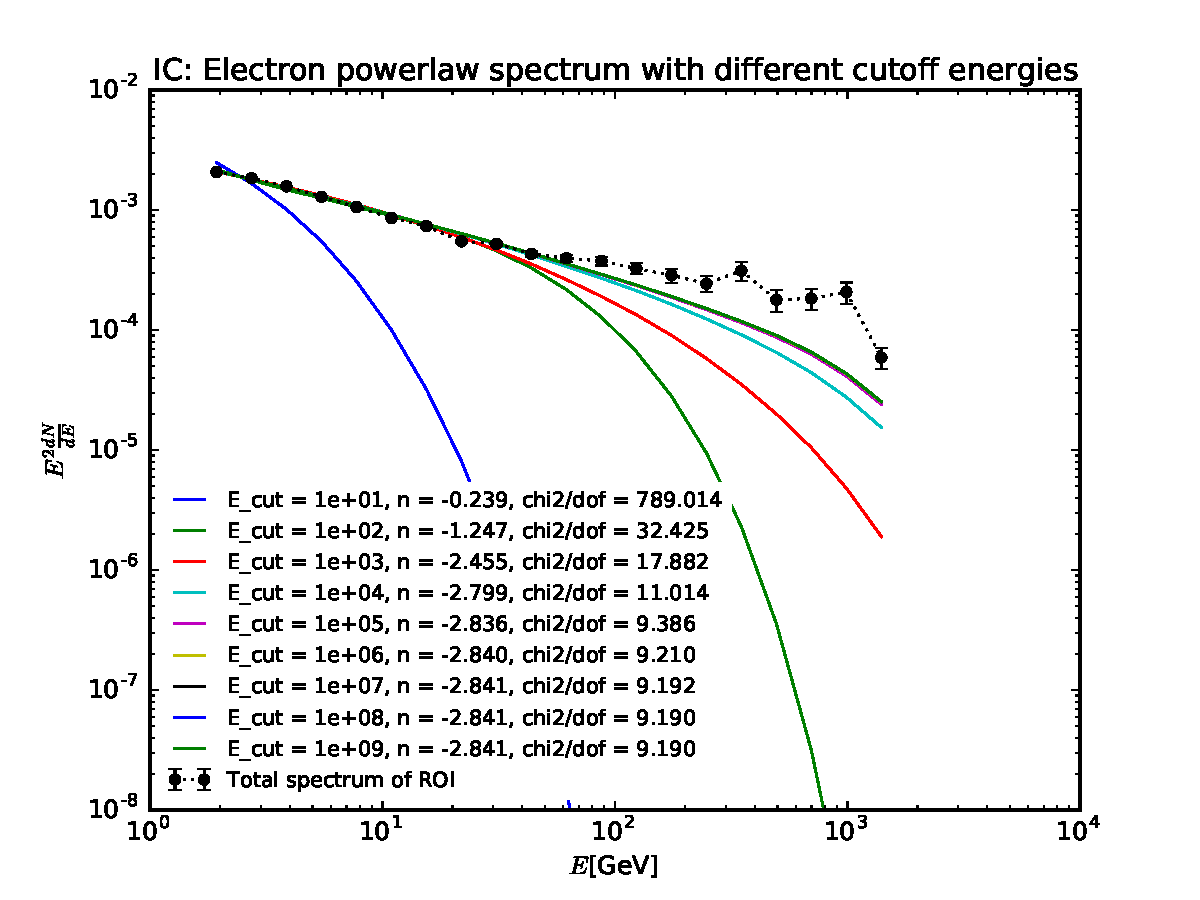
\includegraphics[width=.95\textwidth]{Compare_IC_Ecut_of_tot_data.pdf}
	\end{subfigure}%
	\hspace*{-1.2cm}
	\begin{subfigure}[b]{.65\textwidth}
		\centering
		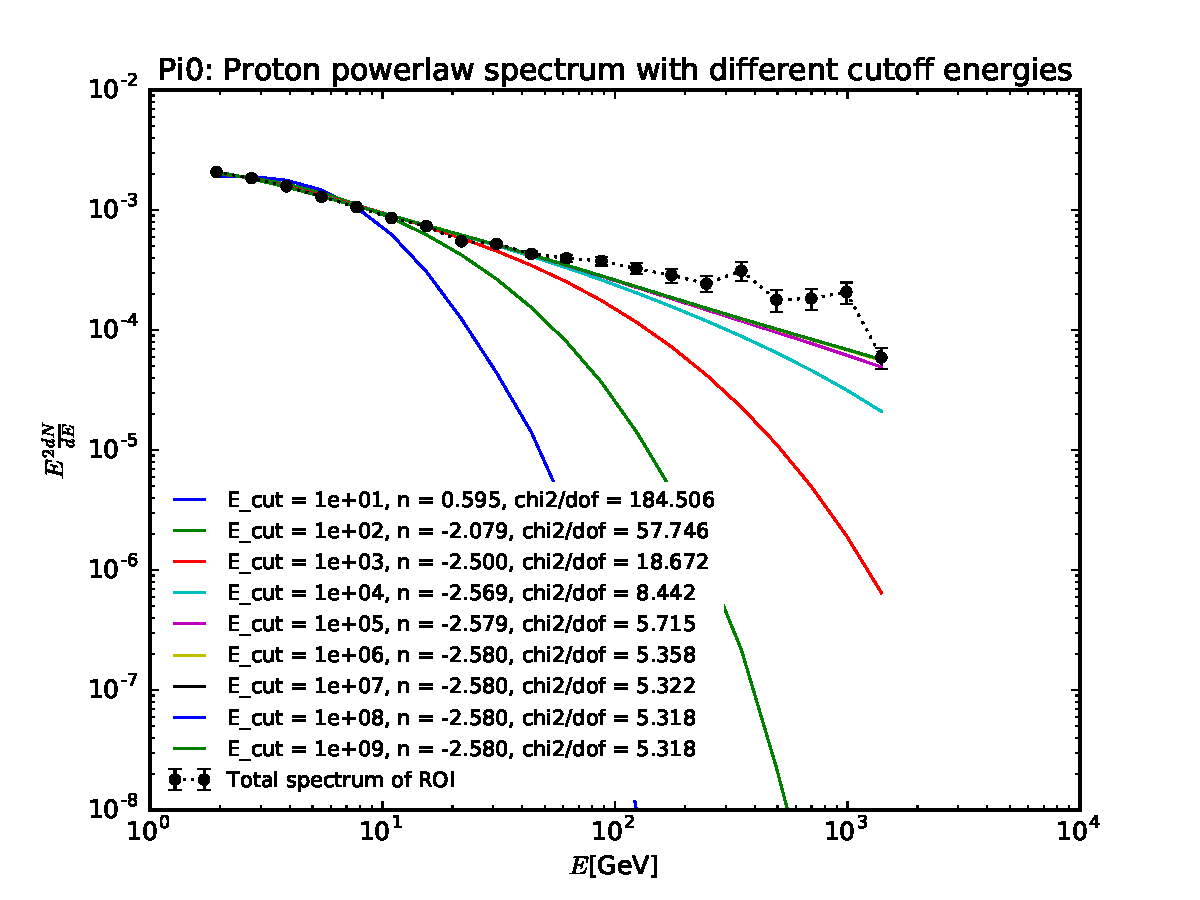
\includegraphics[width=.95\textwidth]{Compare_pi0_Ecut_of_tot_data.pdf}
	\end{subfigure}%
	}\\
	\makebox[\linewidth][c]{%
	\begin{subfigure}[b]{.65\textwidth}
		\centering
		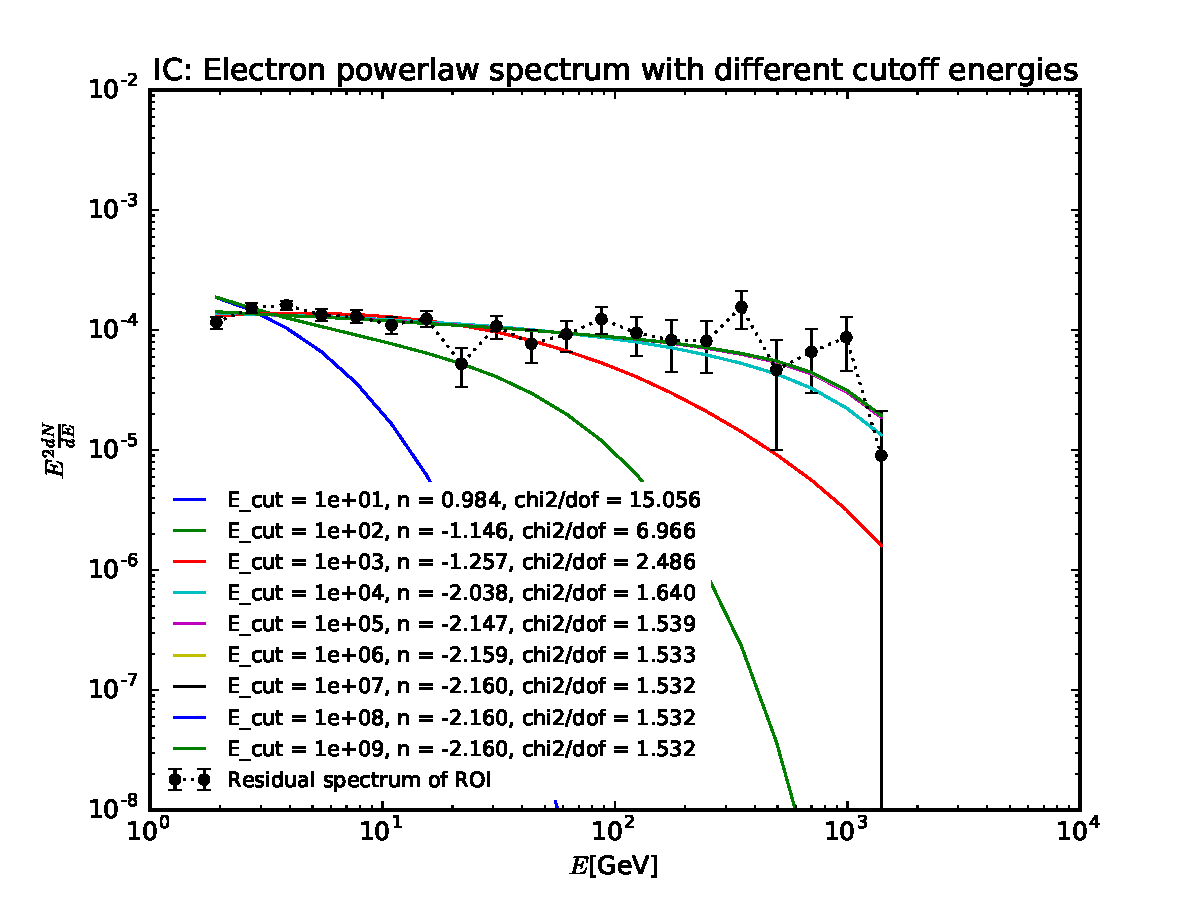
\includegraphics[width=.95\textwidth]{Compare_IC_Ecut_of_res_data.pdf}
	\end{subfigure}%
	\hspace*{-1.2cm}
	\begin{subfigure}[b]{.65\textwidth}
		\centering
		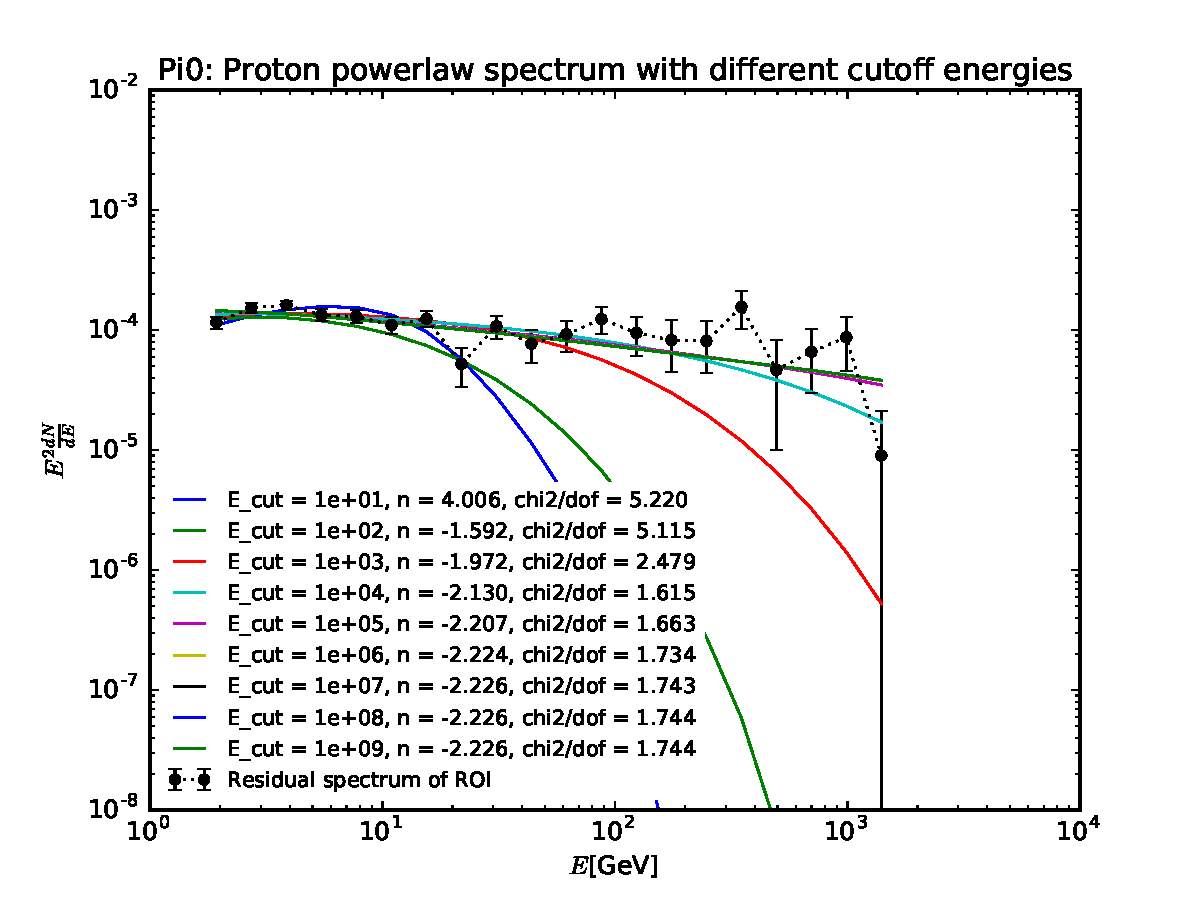
\includegraphics[width=.95\textwidth]{Compare_pi0_Ecut_of_res_data.pdf}
	\end{subfigure}%
	}
\caption{Electron and proton powerlaw spectra with different cutoff energies. The higher the cutoff energy, the better the agreement with the data.}
\label{Cutoff_energies}
\end{figure}









\subsection{Simple calculations of electron and proton lifetimes. Necessary SN rate}


\begin{figure}[h]
%\vspace*{-3cm}
	\centering
	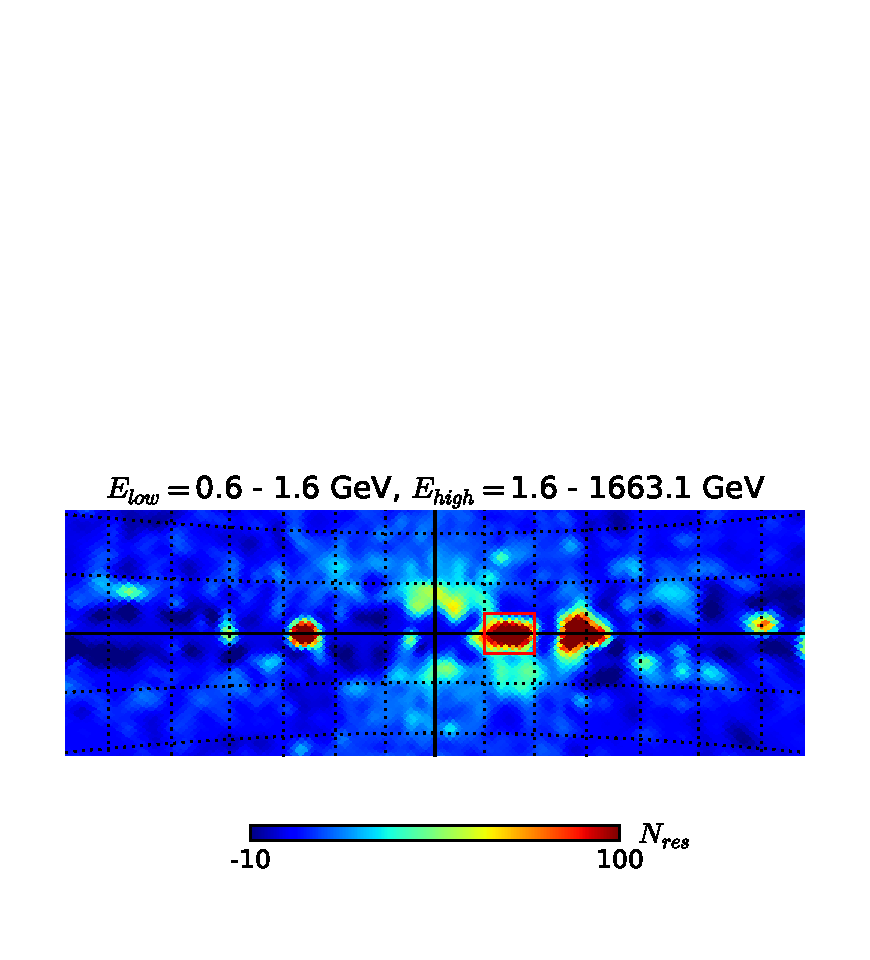
\includegraphics[width=0.5\textwidth]{gnomview_1}
    \caption{Residual photon counts map. The region of interest (ROI) at $b \in (-2^\circ, 2^\circ)$ and $\ell \in (-10^\circ, -4^\circ)$ is marked with a red rectangle, excessive gamma-ray emission is clearly visible. Low-energy \textit{Fermi} data and isotropic background is used as a model, i.e., $N_\text{res} = N_\text{high} - k \cdot N_\text{low} - c$ (bubbles excluded from fit). The center of the map coincides with the Galactic center. The distance between two graticules is $5^\circ$. The map is smoothed with a Gaussian of $5^\circ$ FWHM. Point sources are masked.}
    \label{gnomview}
\end{figure}

\subsubsection{Luminosity of the excess-flux region}
The \textbf{residual} luminosity of the ROI per unit detector area is approximately 
\begin{equation}
\label{eq_dLdA}
\frac{dL}{dA} = \int_\text{ROI} \int_{E_0}^\infty E\ \frac{dN^\gamma}{d\Omega\ dE\ \tau}\ dE\ d\Omega \approx \sum_{i \in \text{ROI}}\ \sum_{j: E_j > E_0}  E_j\ \frac{N_{ij}^\gamma}{\tau_{ij}} = 2.9 \cdot 10^{-10}\ \frac{\text{erg}}{\text{cm}^2\text{s}}
\end{equation}
where $E_j$ is the mean energy of energy bin $j$, $N_{ij}^\gamma$ and $\tau_{ij}$ are the number of photon counts and exposure in pixel $i$ and energy bin $j$, respectively.\\

Assuming that the ROI is close to the Galactic center, as it would be expected if it was related to the \textit{Fermi} bubbles, the total luminosity of the ROI is
\begin{equation}
\label{eq_L}
L = \int_{\substack{\text{Sphere with} \\ \text{radius }R}}\ \frac{dL}{dA}\ dA = 4 \pi R^2\ \frac{dL}{dA} = 2.2 \cdot 10^{36}\ \frac{\text{erg}}{\text{s}}
\end{equation}
with the distance $R = 8$ kpc to the ROI. Expressed in solar luminosities the luminosity becomes $L = 572\ L_\odot$, or expressed in terms of luminosity per area from the Crab nebula $\frac{dL}{dA} = 12 $ mCrab. 


\subsubsection{Cosmic-ray energy density in a purely hadronic model}
Let's assume for now that the excessive gamma-ray emission is produced by neutral pion decay \textbf{only}. How much additional cosmic radiation would be needed to explain the residual gamma radiation from the ROI? (Values and certain formulas are taken from \cite{Longair}.)\\
\\
To calculate the cosmic-ray density $\rho_{\text{CR}}$, we assume the gas density in the ROI to have a typical value for the inner Galaxy, i.e., $\rho_\text{gas} = \frac{1}{\text{cm}^3}$. Since cosmic rays are highly relativistic we can approximate their velocity by the speed of light, $v_\text{CR} = c$. The proton-proton cross section $\sigma_\text{pp} = 2.5 \cdot 10^{-26}$ cm$^2$ for pion production is similar to the geometric size of the proton.\\
Then, the average number of collisions per unit time and area is $P_\text{col} = \rho_{\text{gas}}\ \sigma_{\text{pp}}\ \rho_{\text{CR}}\ v_{\text{CR}}$.\\
However, collisions between cosmic-ray protons and protons or nuclei of the interstellar gas produce not only $\pi^0$ mesons, but also $\pi^+$ and $\pi^-$ mesons. The charged pions decay into muons and further into electrons (and neutrinos). Though, leptons can emit gamma radiation via inverse Compton scattering, this is not taken into account in this calculation. Only the neutral pion decays into two gamma-ray photons. Therefore, only one third of the energy in cosmic rays is converted into gamma radiation. This is expressed in the energy branching ratio $F(E_{\text{CR}}, E_\gamma)$, with $\int F(E_{\text{CR}}, E_\gamma)\ dE_\gamma = \frac{1}{3}E_\text{CR}$.
With that, the luminosity of the ROI can also be written in terms of $P_\text{col}$:
\begin{equation}
\begin{split}
\frac{dL}{dV} &= \int P_\text{col}(E_{\text{CR}}) \int F(E_{\text{CR}}, E_\gamma)\ dE_\gamma\ dE_{\text{CR}}\\
&= \frac{1}{3}\ \rho_{\text{gas}}\ \sigma_{\text{pp}}\ \int \rho_{\text{CR}}\ v_{\text{CR}}\ E_{\text{CR}}\ dE_{\text{CR}}\\
&= \frac{1}{3}\ \rho_{\text{gas}}\ \sigma_{\text{pp}}\ c\ \epsilon_{\text{CR}}
\end{split}
\end{equation}
where $\epsilon_{\text{CR}} = \int \rho_{\text{CR}}\  E_{\text{CR}}\ dE_{\text{CR}}$ is the energy density of cosmic radiation.\\
With the value of the total luminosity $L$ that was calculated in the previous section, one gets for the cosmic-ray energy density:
\begin{equation}
\label{eq_epsilon}
\epsilon_\text{CR} = \frac{3}{\rho_{\text{gas}}\ \sigma_{\text{pp}}\ c}\ \frac{L}{V_\text{ROI}} = 8.8 \cdot 10^{51}\ \frac{\text{erg}}{V_\text{ROI}} = 1.5\cdot 10^{-12}\ \frac{\text{erg}}{\text{cm}^3}. 
\end{equation} 
Thereby, the luminosity $L$ is assumed to be constant over the volume $V_\text{ROI}$ of the ROI. The volume $V_\text{ROI}$ is assumed to have an ellipsoidal shape. The length and height was set to the length and height of the rectangle that is marked in Figure \ref{gnomview} with red lines, assuming a distance of 8 kpc between the ROI and earth. The depth of the ROI is assumed to be the same as the length. This yields the following volume of the ROI:\\
\begin{equation}
V_\text{ROI} = \frac{4}{3}\ \pi\cdot 279 \text{ pc}\cdot (418 \text{ pc})^2 = 0.20 \text{ kpc}^3.
\end{equation}\\
The average energy release of a supernova in cosmic radiation is approximately $E_\text{SNR} \approx 10 ^{49}$ erg. Hence, the cosmic-ray density necessary for the observed luminosity could be explained by around \textbf{880 supernovae}.\\
Assuming an average supernova rate of $\frac{1}{\text{century}}$ in our galaxy, a rough estimate for the supernova rate in a region like the ROI could be $\frac{1}{\text{kyr}}$. Therefore, the timescale in which the ROI has formed, is around 1 Myr. Interestingly, this coincides with the cooling time of the electrons in the \textit{Fermi} bubbles within the leptonic model of Ackermann et al. \cite{Ackermann1}.\\
\\
Another question one could ask is: What would be the distance of the excess when the additional cosmic-ray density was created by one supernova? To answer that question we rearrange Equation \ref{eq_L} and put in Equation \ref{eq_dLdA} and \ref{eq_epsilon}. We get
\begin{equation}
R_\text{1SN} = \sqrt{\frac{L}{4\ \pi\ \frac{dL}{dA}}}\ = \sqrt{\frac{\rho_\text{gas}\ \sigma_\text{pp}\ c\ E_\text{SNR}}{12\ \pi\ \frac{dL}{dA}}}\ = \sqrt{\frac{1}{880}}\cdot 8\ \text{kpc} = 270\ \text{pc}
\end{equation}\\
which is a reasonable distance. Hence, the excess could also be explained by a close-by supernova remnant.








\section{Conclusions}
Prospects for CTA and neutrino telescopes.


\section*{Appendix}
\begin{figure}[h]
	\centering
	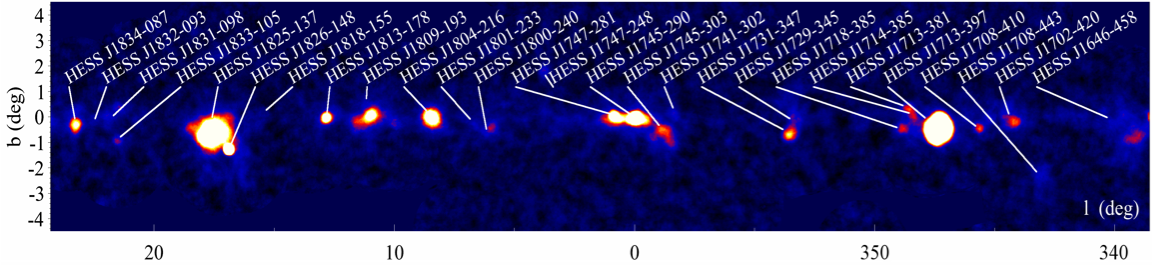
\includegraphics[width=1.\textwidth]{HESS_GalacticPlaneSurvey}
    \caption{H.E.S.S.
     galactic plane survey.}
    \label{TotalData_Sum}
\end{figure}
\begin{figure}[h]
	\centering
	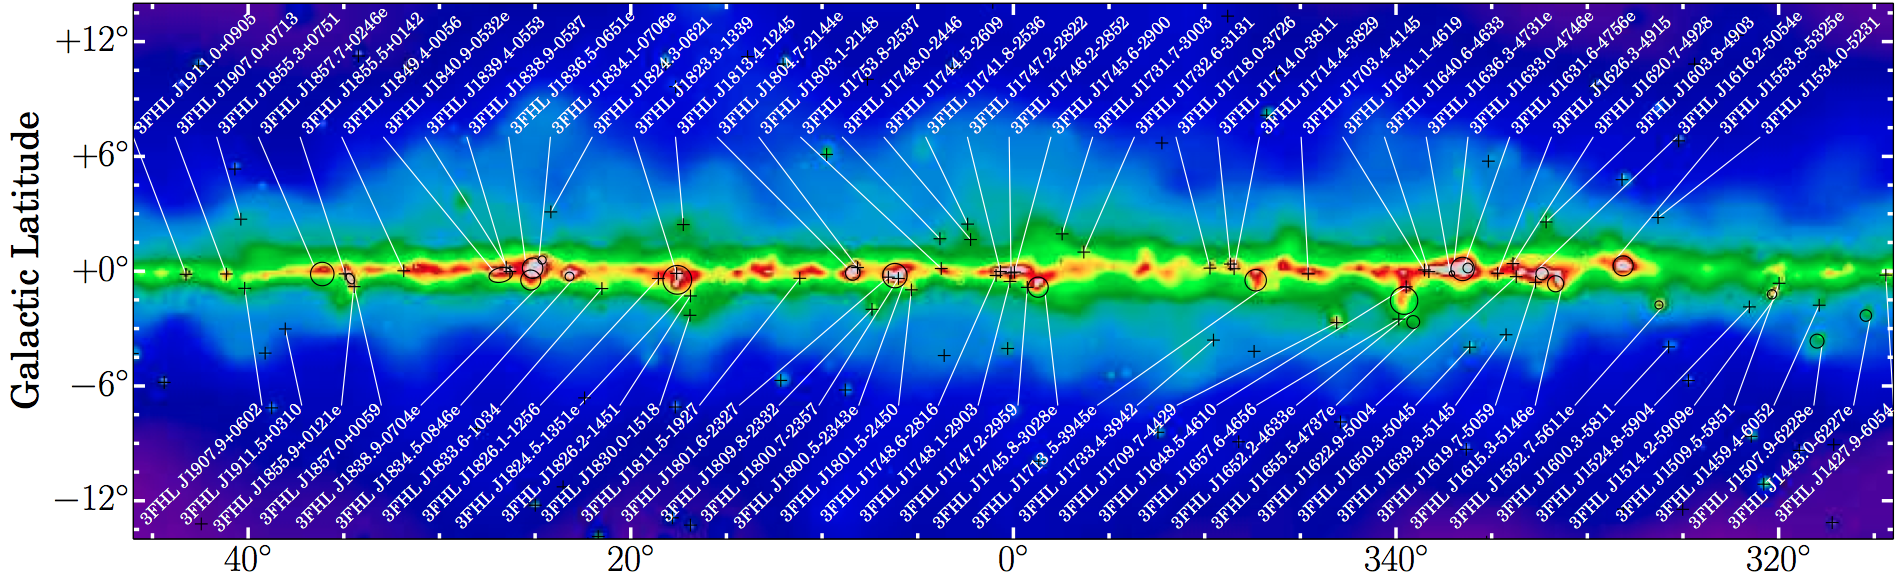
\includegraphics[width=1.\textwidth]{3FHL}
    \caption{Galactic plane with hard sources of the 3FHL cataloge.}
    \label{TotalData_Sum}
\end{figure}



\begin{thebibliography}{9}
	\bibitem{Longair} M. S. Longair. \textit{High Energy Astrophysics}. Cambridge University Press, Cambridge, 3rd edition (2011).
	\bibitem{Ackermann1} M. Ackermann, A. Albert, W. B. Atwood et al. \textit{The Spectrum and Morphology of the \textit{Fermi} Bubbles}. arXiv:1407.7905v1 (2014).\\
\end{thebibliography}

\end{document}
